\documentclass[a4paper,11pt]{report}
\usepackage[utf8x]{inputenc}
\usepackage[portuges,english]{babel}
\usepackage{graphicx}
\usepackage{color}
\definecolor{bordo}{RGB}{192,0,0} %--Cor fancy que eu gosto!
\usepackage{makeidx}
\usepackage{caption}
\usepackage{subcaption}
\usepackage{indentfirst}
\usepackage{verbatim}
\usepackage{amsmath}
\usepackage{graphicx}
\usepackage{setspace}
\newcommand{\HRule}{\rule{\linewidth}{0.5mm}}
\usepackage{trajan}
\usepackage{fetamont}
\usepackage{duerer}
\usepackage{lmodern}
\usepackage[T1]{fontenc}
\usepackage{mathtools}
\usepackage{graphicx,wrapfig,lipsum}
\usepackage{framed}
\usepackage{capt-of}
\usepackage{gensymb}
\usepackage{mdframed}
\usepackage{xcolor}
\usepackage{tikz}
\usetikzlibrary{calc}
\usepackage{empheq}
\usepackage{nameref} %Para utilizar nameref
\usepackage[makeroom]{cancel}
\usepackage{amssymb} %para poder usar \leqslant no math mode
\usepackage{fancyhdr} %-estilo da pagina
%\usepackage{showframe}
\usepackage[margin=2.5cm]{geometry}
\usepackage[hypertexnames=false]{hyperref}
\usepackage{multirow}
\usepackage{pdfpages}
\usepackage{lscape} %para usar página horizontal
\usepackage{multicol} %para poder por 3 figuras alinhas
\usepackage{cases}
\usepackage{hhline}
\usepackage{float}

%%% - Caso queira utilizar anexos
\newcommand{\annexname}{Annex}
\makeatletter
\newcommand\annex{\par
  \setcounter{chapter}{0}%
  \setcounter{section}{0}%
  \gdef\@chapapp{\annexname}%
  \gdef\thechapter{\@Roman\c@chapter}}
\makeatother

%%%   Para que os capitulos so tenham o titulo e nao a numeraçao de capitulo%%%%%%
  \usepackage{titlesec}
  \titleformat{\chapter}
  {\Large\bfseries} % format
  {}                % label
  {0pt}             % sep
  {\Huge}           % before-code
  
 
  
\hypersetup{
    pdftitle={Electronica Geral},    % title
    pdfauthor={Afonso Mendes, David Escudeiro, Élio Pereira, Pedro Pinto},     % author
    }



\newcommand{\parallelsum}{\mathbin{\!/\mkern-5mu/\!}} %para usar o simbolo de paralelo em circuitos


%-Poupar papel
%%%%%\setlength{\headheight}{12pt}
%%%%%\setlength{\voffset}{-50pt}
%\setlength{\hoffset}{-72.27pt}
%%%%%\setlength{\textheight}{692pt}
%%%%%\setlength{\footskip}{30pt}
%\setlength{\marginparwidth}{0pt}
%%%%%\setlength{\marginparsep}{0pt}
%%%%%\setlength{\textwidth}{450pt}
%%%%%\setlength{\oddsidemargin}{0pt}
%%%%%\setlength{\evensidemargin}{0pt}
%%%%%\setlength{\marginparsep}{0pt}






%---------------------COMEÇA O DOCUMENTO---------------------%
%---------------------COMEÇA O DOCUMENTO---------------------%
%---------------------COMEÇA O DOCUMENTO---------------------%
%---------------------COMEÇA O DOCUMENTO---------------------%
%---------------------COMEÇA O DOCUMENTO---------------------%

\begin{document}
	\selectlanguage{portuges}
	
 
\begin{titlepage}

	\begin{flushleft}
	
\includegraphics[width=0.6\textwidth]{./logo}~\\[4cm]
	\end{flushleft}

\begin{center}
\begin{spacing}{2}

	\textsc{\LARGE Electrónica Geral}\\[1cm]

\HRule \\[0.4cm]
{ \huge \bfseries Filtro Adaptativo}\\[0.4cm]

\HRule \\[1.5cm]

\end{spacing}

	\vspace{2cm}

	Afonso Mendes, \quad 75398\\
	David Escudeiro \quad 75479\\
	Élio Pereira, \quad 78535\\
	Pedro Pinto, \quad 75239\\
	\vspace{4cm}


\vfill

{\large 4 de Dezembro de 2015}
\end{center}
\end{titlepage} 





\addtocontents{toc}{\protect\thispagestyle{empty}} %para nao ter numeraçao de pagina na pagina da ToC
\tableofcontents %put toc in
%\setcounter{secnumdepth}{-2} %para as secçoes nao apresentarem numero no indice
%\cleardoublepage %start new page
\setcounter{page}{1} %reset the page counter
%%-estilo da pagina
%\pagestyle{fancy}
%\renewcommand{\headrulewidth}{2pt} 
%\lhead[Electrónica Geral]{Electrónica Geral}
%\chead[]{}
%\rhead[Filtros Activos e Osciladores]{Filtros Activos e Osciladores}
%\lfoot[]{}
%\cfoot[\thepage]{\thepage}
%\rfoot[]{}


%%%%%%%%%%%%%%%%%%%%%%%%%%%%%%%%%%%%%%%%%%%%%%%%%%%%%%%%%%%%%%%%%%%%%%%%%%%%%%%%%%%%%%%%%%%%%%%%%

\chapter{Introdução}

Neste trabalho laboratorial será desenvolvido um esquema de implementação e simulação de um sistema de comunicação em banda de base com o intuito de estudar o comportamento de um filtro adaptativo FIR transversal executado pelo algoritmo LMS a operar como cancelador de eco.\\

Sequencialmente, serão apresentadas neste relatório as concepções dos diferentes constituintes do sistema a simular acompanhadas dos testes correspondentes que permitem a verificação do seu correcto funcionamento. Numa parte final do trabalho, o sistema será testado na sua totalidade de forma a gerar conclusões relativamente à estabilidade do algoritmo implementado e à velocidade de convergência do mesmo.\\

Apresenta-se na figura seguinte a arquitectura do sistema a implementar.

\begin{center}
     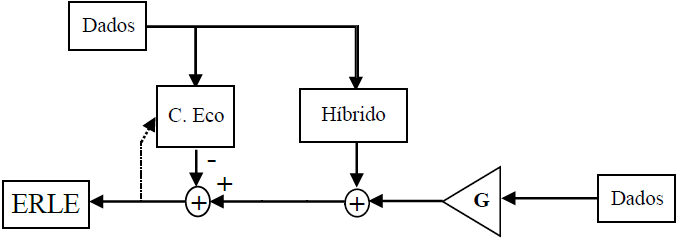
\includegraphics[angle=0,width=0.9\textwidth]{arqui.png}
     \captionof{figure}{ Arquitectura do sistema de comunicação a simular.}
     \label{fig:arqui}
\end{center}

\chapter{Baralhador de Dados}
\section{Implementação}

Para gerar os dados aleatórios, quer do emissor local, quer do emissor remoto, usa-se um gerador de onda quadrada seguido de um baralhador de dados. O baralhador utilizado corresponde ao polinómio $1+x^3+x^5$ no caso do emissor local, e $1+x^5+x^7$ no caso do emissor remoto, a que correspondem, respectivamente, as seguintes operações:
$$y(t)=x(t)\oplus y(t-3T)\oplus y(t-5T)$$
$$y(t)=x(t)\oplus y(t-5T)\oplus y(t-7T)$$

sendo T o período dos dados e $\oplus$ o operador lógico ``ou-exclusivo (XOR)''. Para realizar estas operações, foi feito, no \textit{Simulink}, os diagramas de blocos apresentados na Figura \ref{fig:gerador_dados_local} para o gerador de dados local, e na Figura \ref{fig:gerador_dados_remoto} para o remoto. O bloco ``\textit{Pulse Generator}'' é o que gera o sinal $x(t)$.

\begin{center}
     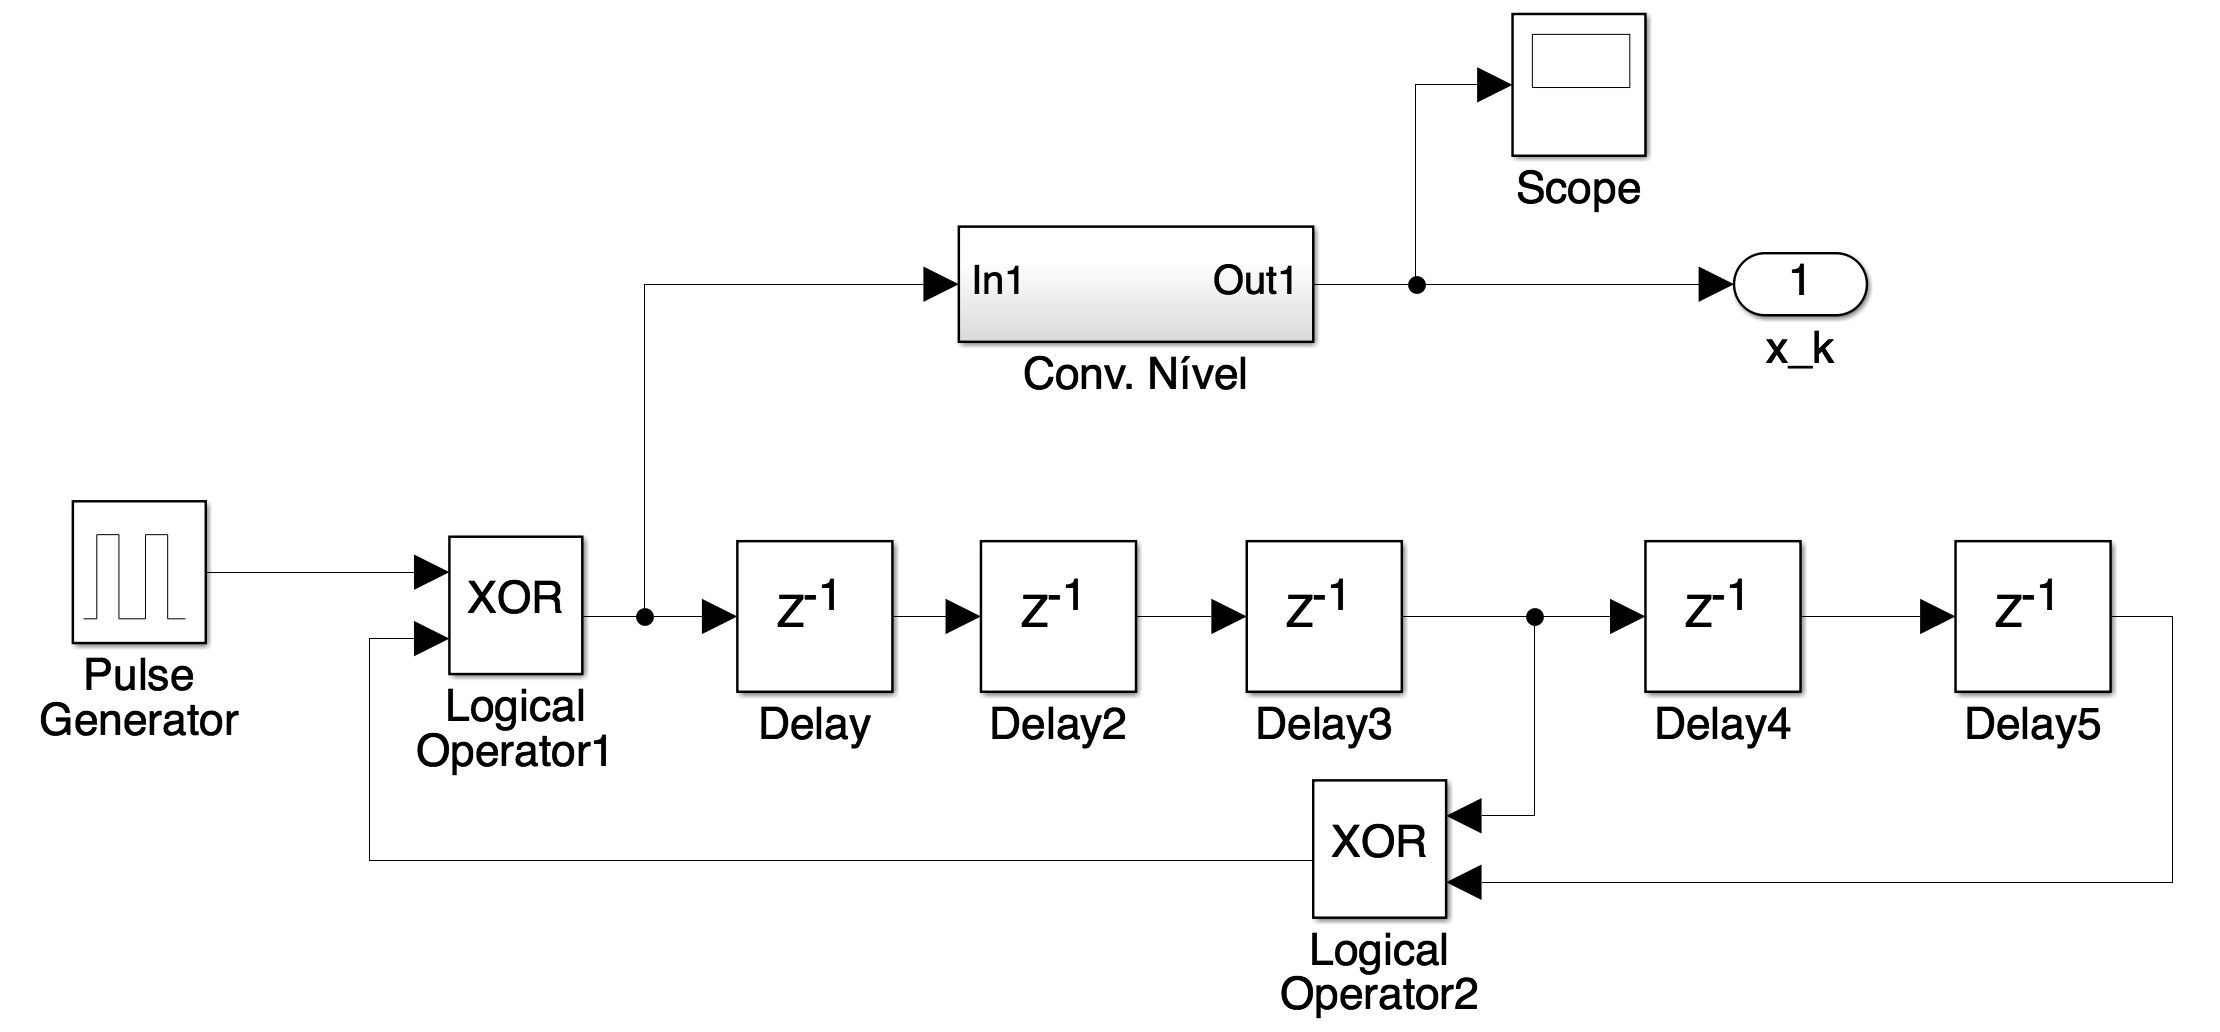
\includegraphics[angle=0,width=1.0\textwidth]{gerador_dados_local.png}
     \captionof{figure}{ Diagrama de blocos do baralhador de dados local.}
     \label{fig:gerador_dados_local}
\end{center}

\begin{center}
     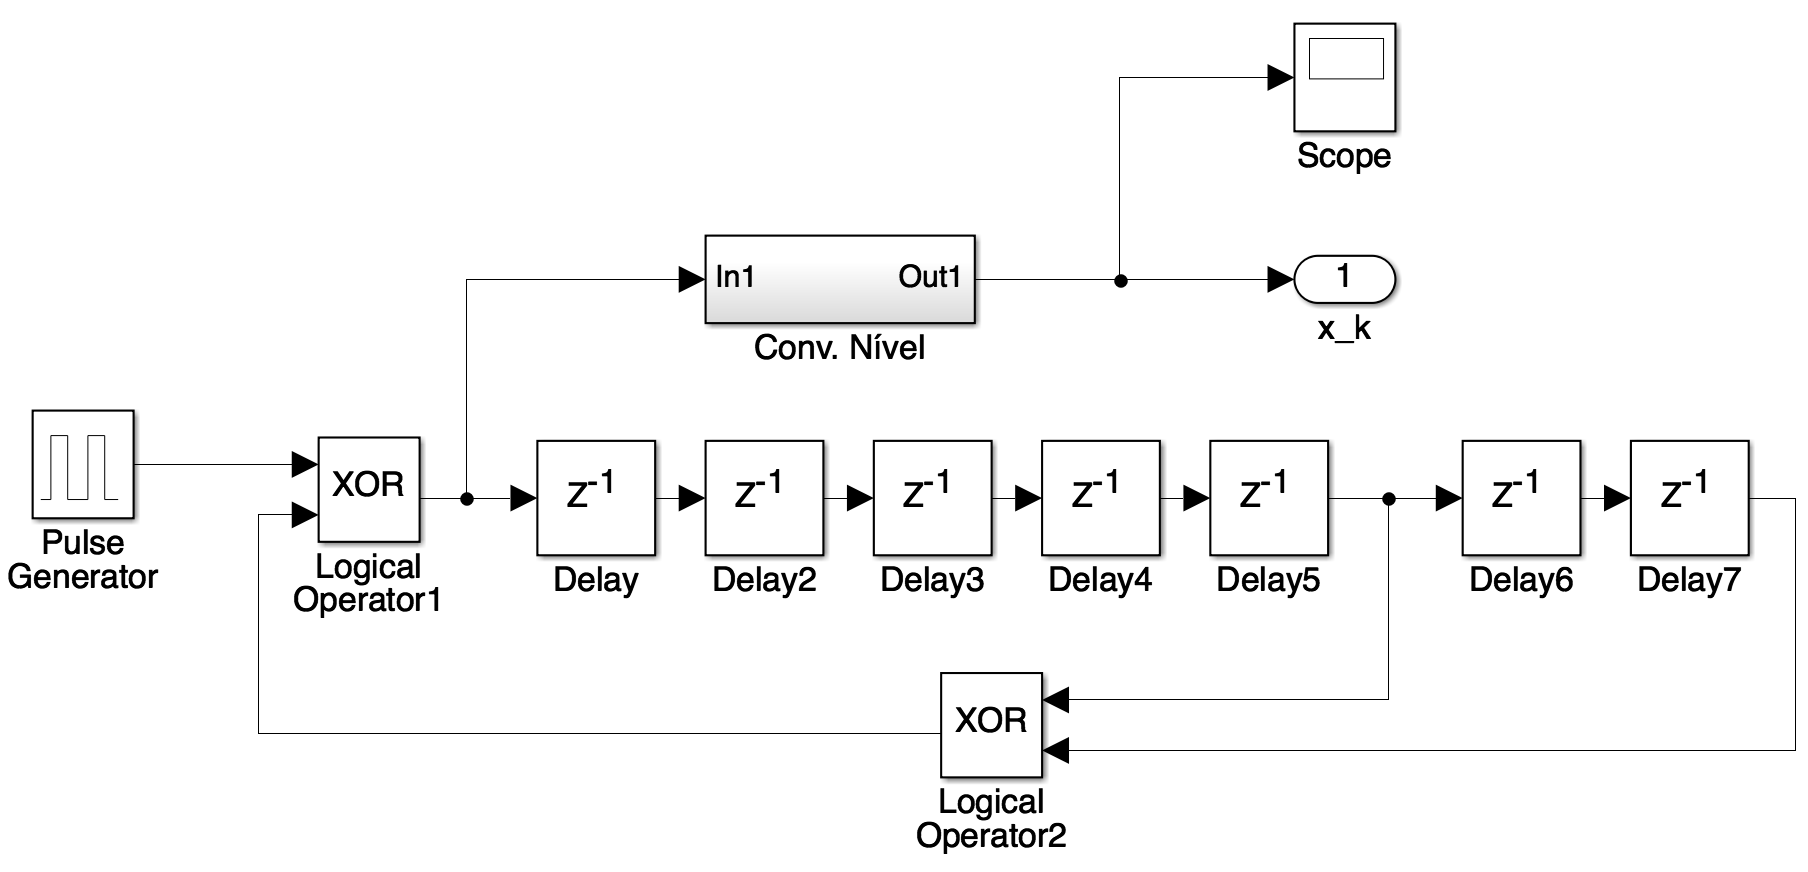
\includegraphics[angle=0,width=1.0\textwidth]{gerador_dados_remoto.png}
     \captionof{figure}{ Diagrama de blocos do baralhador de dados remoto.}
     \label{fig:gerador_dados_remoto}
\end{center}

Em ambos os casos, o bloco Conversor de nível, ``\textit{Conv. Nível}'', corresponde ao diagrama apresentado na Figura \ref{fig:conversor_nivel}:

\begin{center}
     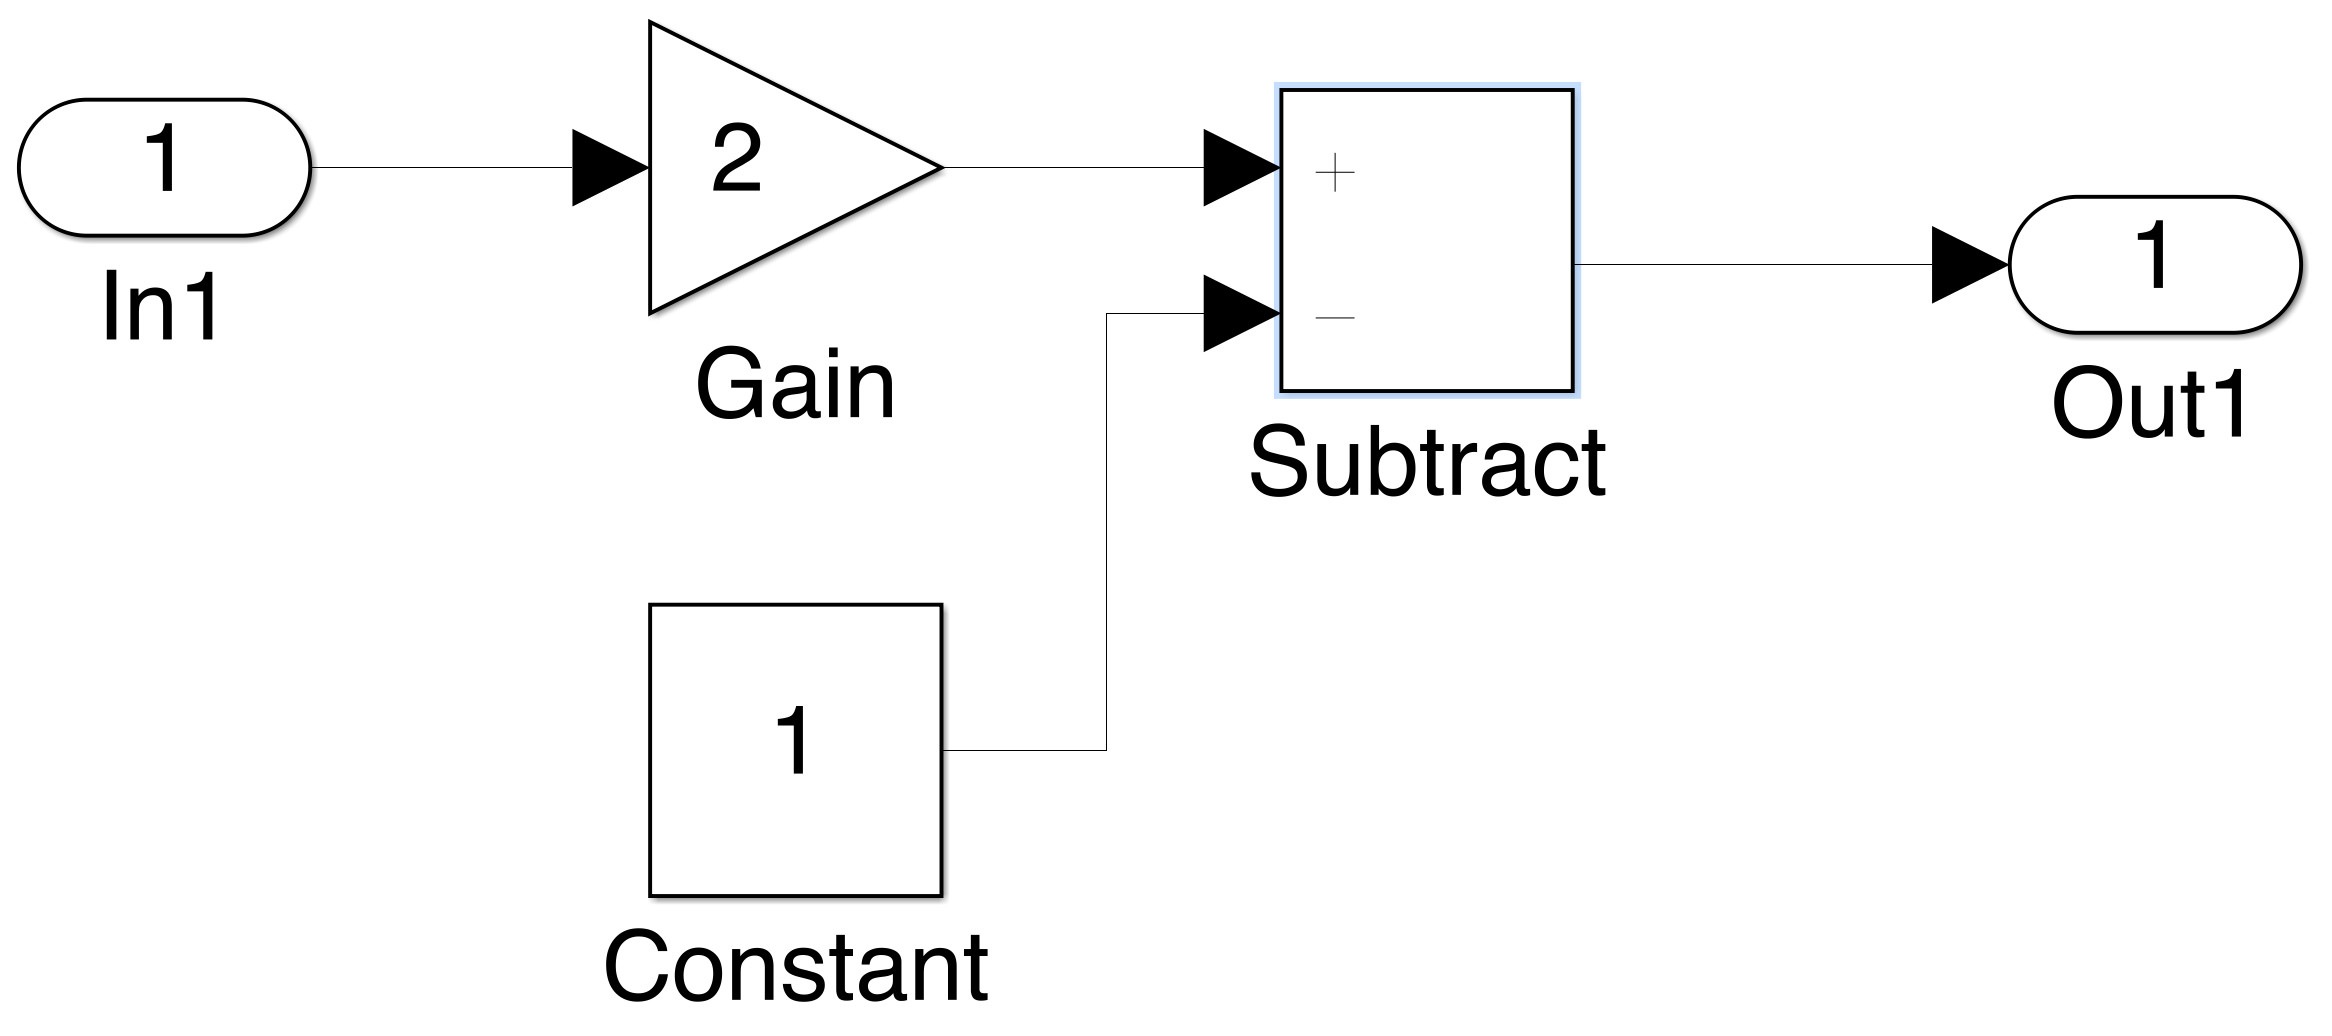
\includegraphics[angle=0,width=0.5\textwidth]{conversor_nivel.png}
     \captionof{figure}{ Diagrama de blocos do conversor de nível.}
     \label{fig:conversor_nivel}
\end{center}

\section{Teste e Análise}
\par

\large\underline{{\textit{\textbf{Gerador de dados local}}}}\\
\par

Para testar o baralhador de dados, introduzimos uma onda quadrada de frequência 2T, uma vez que cada período desta onda vai gerar dois sinais, um de nível ``\textit{High}'' e outro ``\textit{Low}'', cada um de duração T. A amplitude da onda quadrada utilizada foi 1 Volt, e $T=1$ s. 
Apresenta-se na Figura \ref{fig:grafico_5_1_1} o sinal de entrada aplicado à entrada do baralhador de dados, e na Figura \ref{fig:grafico_5_1_2} o sinal de saída do mesmo.

\begin{minipage}[t]{0.5\textwidth}
  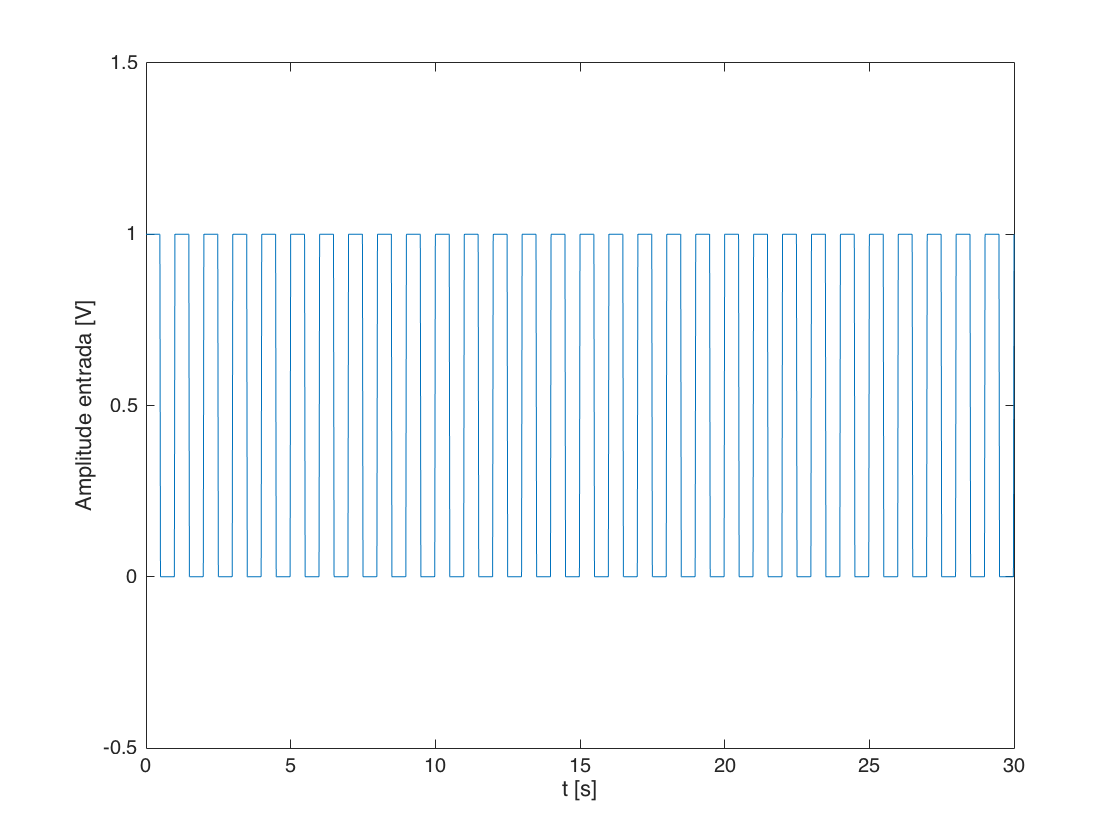
\includegraphics[angle=0,width=1\textwidth]{grafico_5_1_1.png}
     \captionof{figure}{Sinal de entrada do baralhador de dados local}
     \label{fig:grafico_5_1_1}
     \end{minipage}%
\hspace{0.3cm}
\begin{minipage}[t]{0.5\textwidth}
  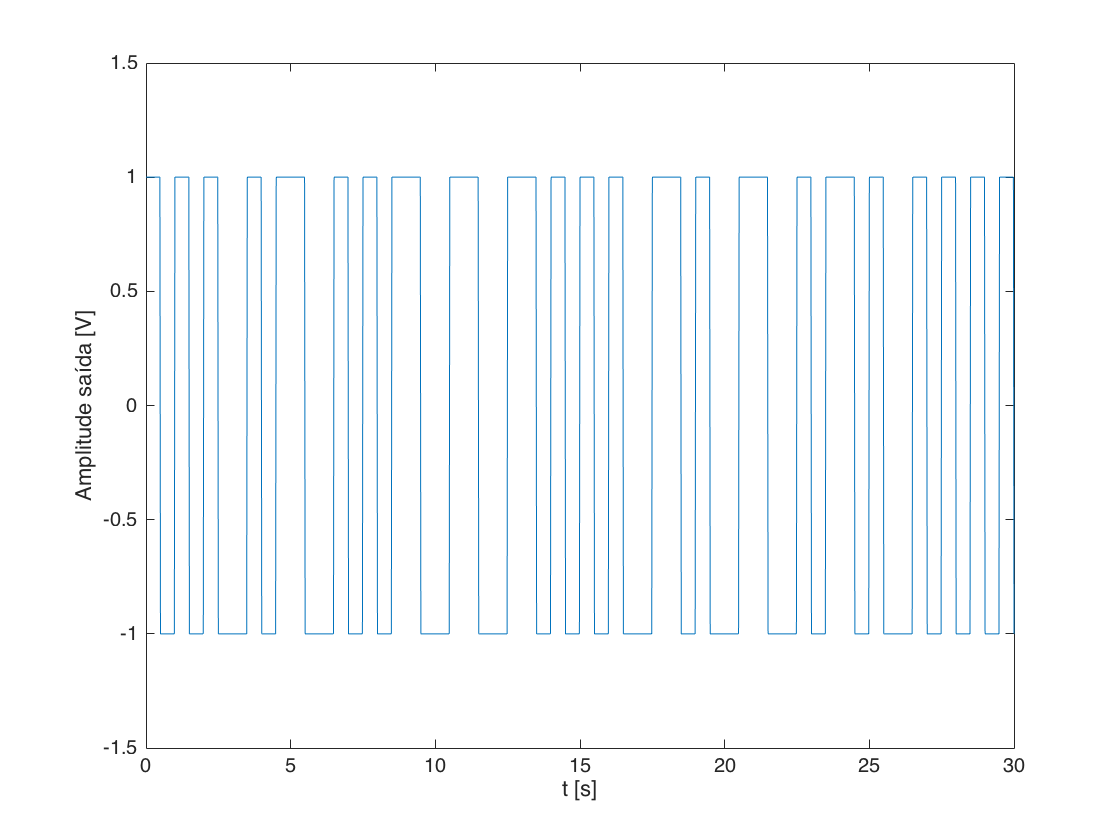
\includegraphics[angle=0,width=1\textwidth]{grafico_5_1_2.png}
    \captionof{figure}{Sinal de saída do baralhador de dados local}
     \label{fig:grafico_5_1_2}
     \end{minipage}\\
     
Observa-se claramente o efeito do baralhador de dados, sendo o sinal gerado pseudo-aleatório. Também se pode observar o efeito do conversor de nível, uma vez que o sinal passa de [0,1] V para [-1,1] V.

De seguida foi introduzido um sinal de dados de entrada permanentemente a zero, em vez da onda quadrada. Apresenta-se este sinal, bem como o sinal de saída, nas Figuras \ref{fig:grafico_5_1_3} (sinal de entrada) e \ref{fig:grafico_5_1_4} (sinal de saída):

\begin{minipage}[t]{0.5\textwidth}
  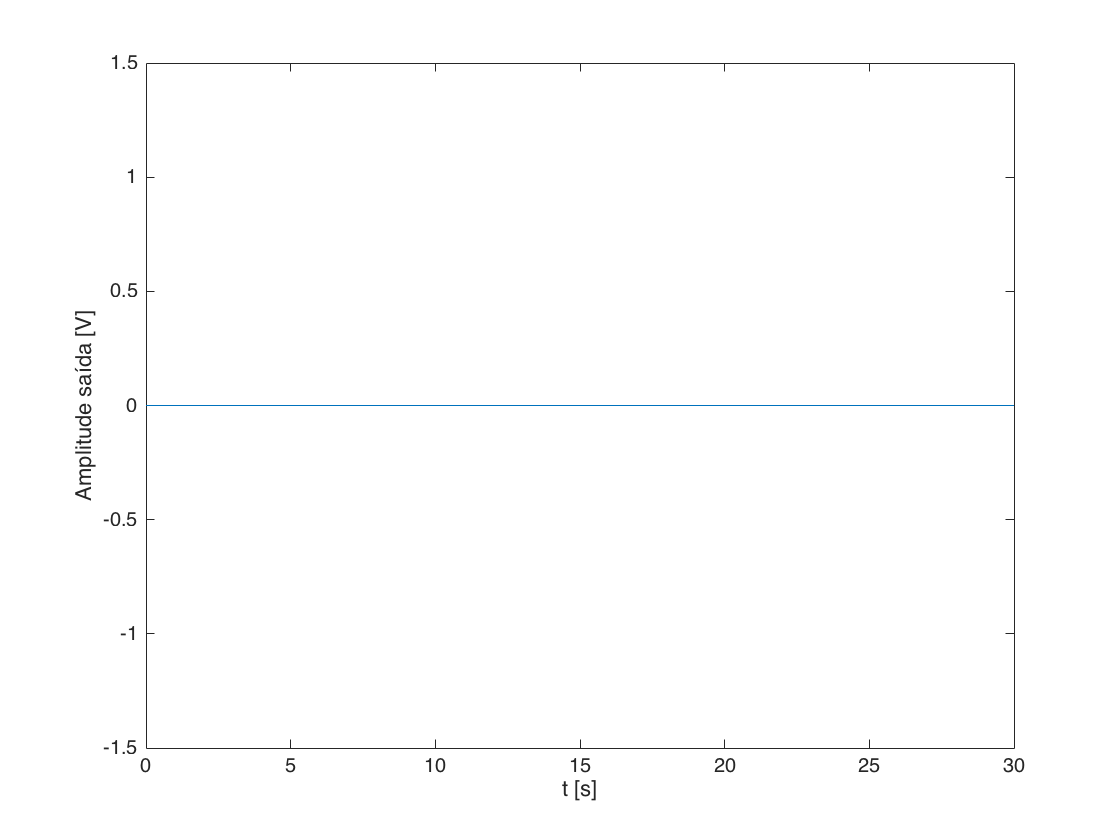
\includegraphics[angle=0,width=1\textwidth]{grafico_5_1_3.png}
     \captionof{figure}{Sinal de entrada do baralhador de dados local}
     \label{fig:grafico_5_1_3}
     \end{minipage}%
\hspace{0.3cm}
\begin{minipage}[t]{0.5\textwidth}
  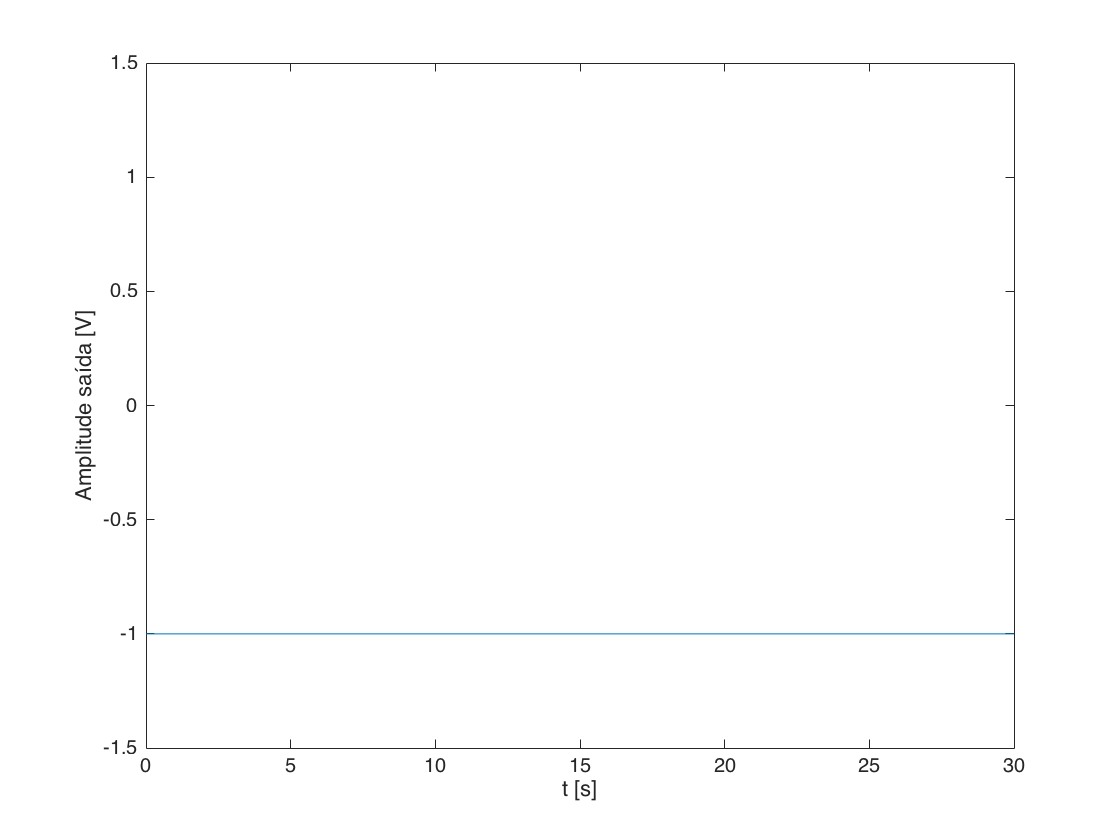
\includegraphics[angle=0,width=1\textwidth]{grafico_5_1_4.png}
    \captionof{figure}{Sinal de saída do baralhador de dados local}
     \label{fig:grafico_5_1_4}
     \end{minipage}\\

Neste caso o sinal de saída é contínuo e igual a -1 V. Isto acontece uma vez que, sendo o sinal de entrada contínuo a 0 V, e as condições iniciais também nulas, ao passar pelos operadores lógicos ``ou-exclusivo (XOR)'', dá-se a operação $0\oplus 0=0$. O sinal de saída é -1, devido ao conversor de nível que transforma o 0 em -1.\\
\par

\large\underline{{\textit{\textbf{Gerador de dados remoto}}}}\\
\par

No caso do gerador de dados remoto, foi introduzida a mesma onda quadrada como sinal de entrada, tendo sido obtido um sinal pseudo-aleatório diferente, que se apresenta na Figura \ref{fig:grafico_5_1_6}:

\begin{minipage}[t]{0.5\textwidth}
  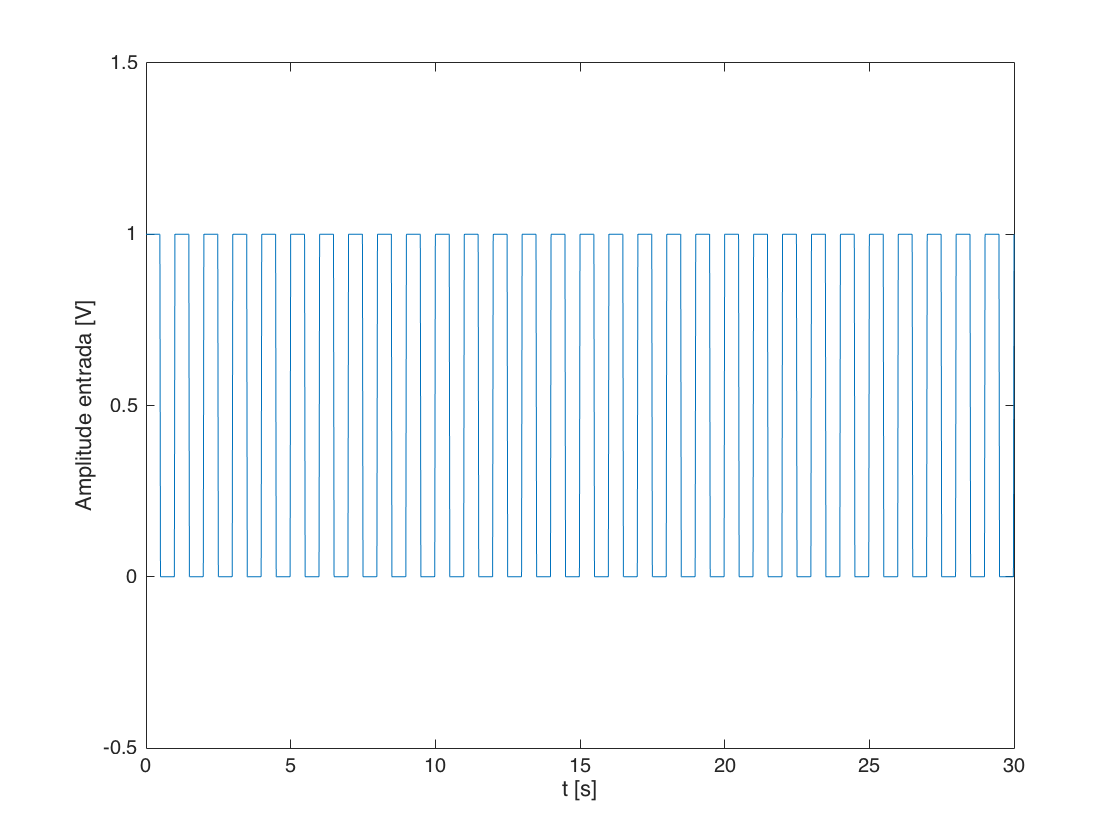
\includegraphics[angle=0,width=1\textwidth]{grafico_5_1_5.png}
     \captionof{figure}{Sinal de entrada do baralhador de dados remoto}
     \label{fig:grafico_5_1_5}
     \end{minipage}%
\hspace{0.3cm}
\begin{minipage}[t]{0.5\textwidth}
  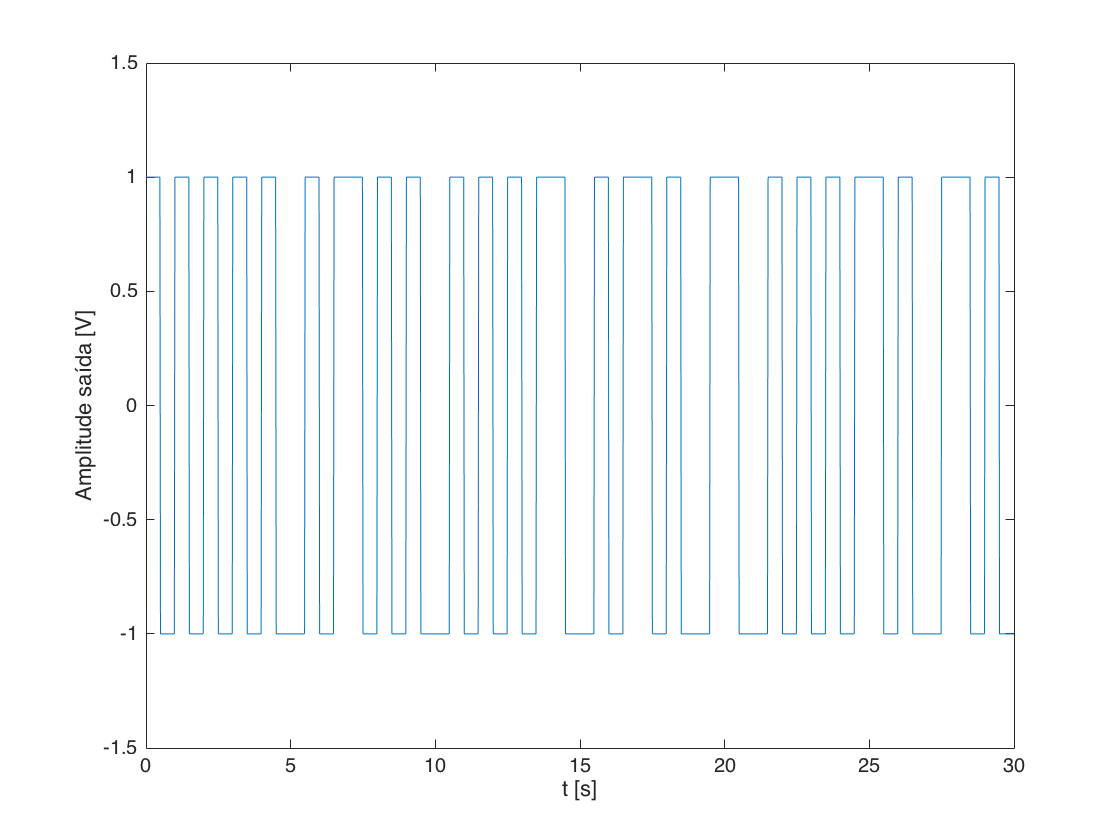
\includegraphics[angle=0,width=1\textwidth]{grafico_5_1_6.png}
    \captionof{figure}{Sinal de saída do baralhador de dados remoto}
     \label{fig:grafico_5_1_6}
     \end{minipage}\\
     
De seguida foi aplicado o sinal de entrada contínuo a 0 V, tendo sido obtido o mesmo sinal que no caso do gerador de dados local com o mesmo sinal de entrada, pelas razões apresentadas anteriormente. Apresenta-se então o sinal de entrada, Figura \ref{fig:grafico_5_1_7}, e de saída, Figura \ref{fig:grafico_5_1_8}, do baralhador de dados remoto com a entrada a 0 V:

\begin{minipage}[t]{0.5\textwidth}
  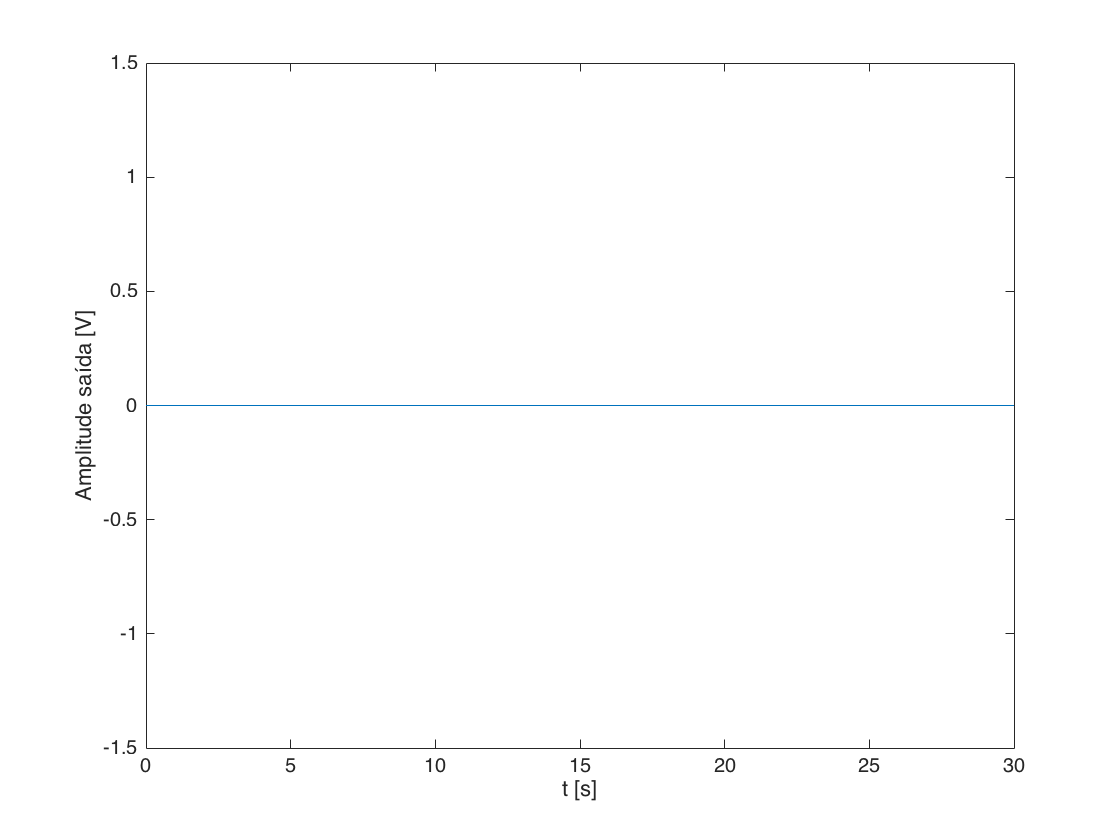
\includegraphics[angle=0,width=1\textwidth]{grafico_5_1_7.png}
     \captionof{figure}{Sinal de entrada do baralhador de dados remoto}
     \label{fig:grafico_5_1_7}
     \end{minipage}%
\hspace{0.3cm}
\begin{minipage}[t]{0.5\textwidth}
  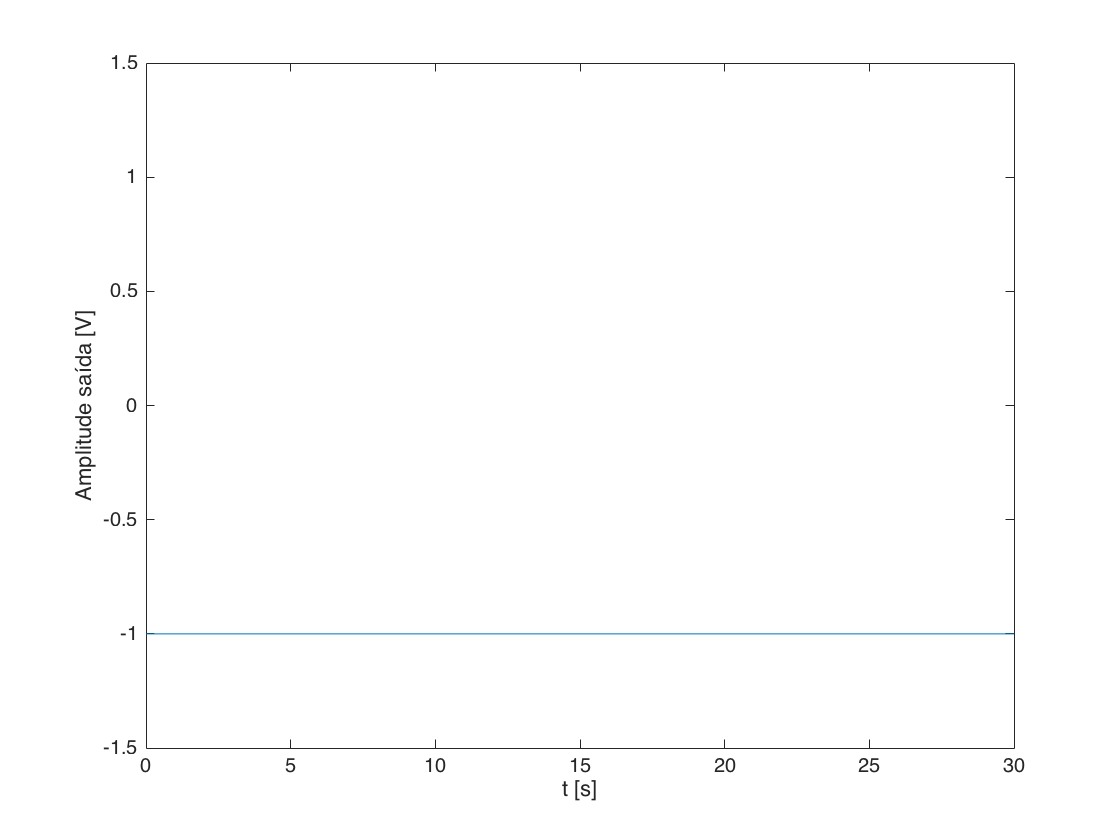
\includegraphics[angle=0,width=1\textwidth]{grafico_5_1_8.png}
    \captionof{figure}{Sinal de saída do baralhador de dados remoto}
     \label{fig:grafico_5_1_8}
     \end{minipage}\\

\chapter{Híbrido}
\section{Implementação}
Uma vez que este sistema de transmissão de dados funciona a 4 fios para os emissores e recetores e a 2 fios na linha de transmissão, é necessário utilizar um circuito chamado \textit{híbrido} para fazer esta transição. Neste caso, para simular um híbrido, usou-se um filtro FIR (\textit{Finite Impulse Response}) transversal de 9ª ordem, com uma resposta impulsional do tipo $sinc(x)=sen(x)/x$, que se apresenta na seguinte Figura \ref{fig:hibrido}:

\begin{center}
     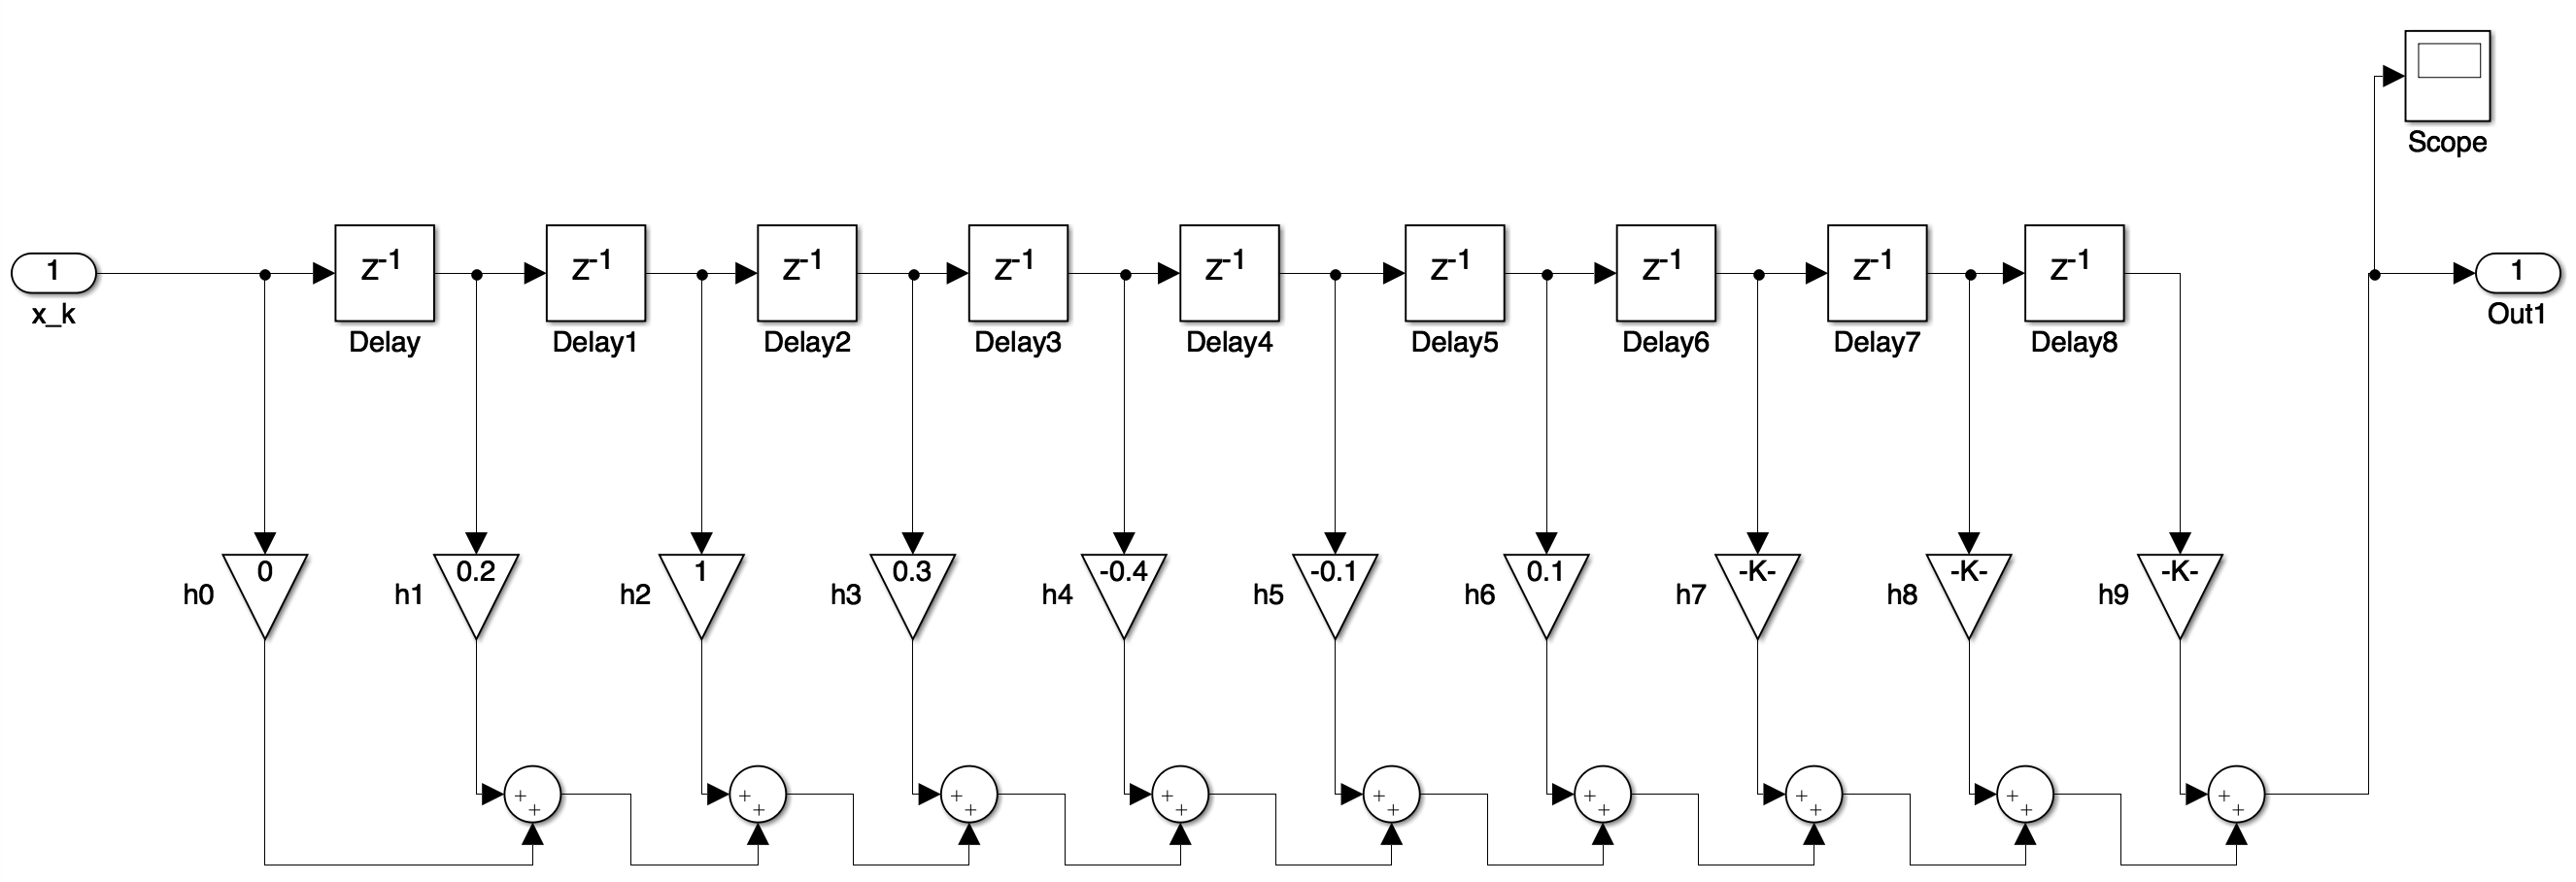
\includegraphics[angle=0,width=1\textwidth]{hibrido.png}
     \captionof{figure}{Diagrama de blocos do híbrido}
     \label{fig:hibrido}
\end{center}

Os coeficientes $e_i$, $i=0,1,...,9$, utilizados no diagrama de blocos do híbrido são os que se encontram na Tabela \ref{tab:coeficientes_hibrido}:

\begin{table}[h]
\centering
\begin{tabular}{ || c | c | c | c | c | c | c | c | c | c || }
\hline
	$e_o$ & $e_1$ & $e_2$ & $e_3$ & $e_4$ & $e_5$ & $e_6$ & $e_7$ & $e_8$ & $e_9$ \\ \hline  \hline
	0 & 0.2 & 1 & 0.3 & -0.4 & -0.1 & 0.1 & -0.05 & -0.02 & -0.01 \\ \hline
\end{tabular}

\caption{Coeficientes do filtro FIR que representa o híbrido \label{tab:coeficientes_hibrido}}

\end{table}

\section{Teste e Análise}

Para o teste deste bloco híbrido foi colocado um sinal unitário contínuo à sua entrada, tendo sido obtido um sinal de saída que se apresenta na figura \ref{fig:grafico_5_3}:

\begin{center}
     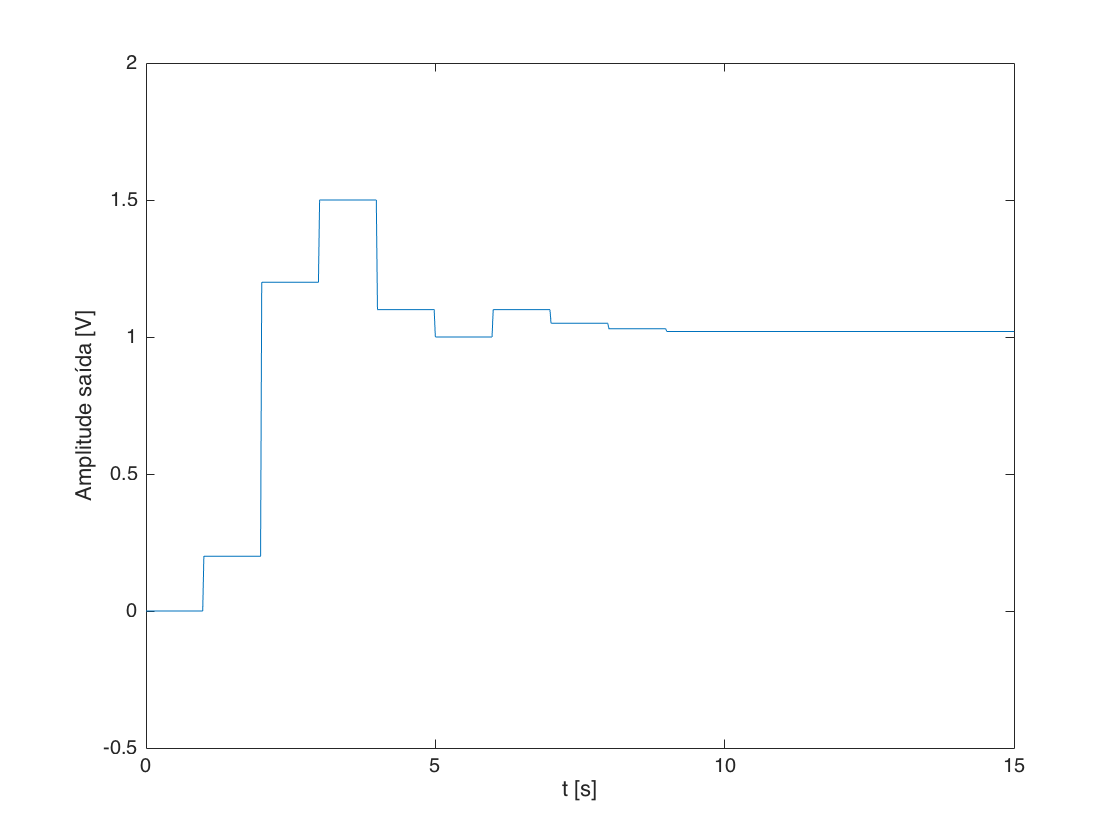
\includegraphics[angle=0,width=0.8\textwidth]{grafico_5_3.png}
     \captionof{figure}{Sinal de saída do híbrido}
     \label{fig:grafico_5_3}
\end{center}

Observando esta resposta ao sinal contínuo de nível 1, pode-se constatar logo à partida a estabilidade inerente de um filtro FIR. 

Para uma análise mais detalhada vai-se calcular a função de transferência e respetiva representação no plano Z:

$$y(t)=0.2x(t-1)+x(t-2)+0.3x(t-3)-0.4x(t-4)-0.1x(t-5)+$$
$$+0.1x(t-6)-0.05x(t-7)-0.02x(t-8)-0.01x(t-9)$$
$$\Rightarrow \frac{y(t)}{x(t)}=\frac{0.2z^8+z^7+0.3z^6-0.4z^5-0.1z^4+0.1z^3-0.05z^2-0.02z-0.01}{z^{9}}+$$

A esta função de transferência correspondem os seguintes zeros, representados no plano Z na Figura \ref{fig:grafico_5_3_zplane}:

\begin{center}
     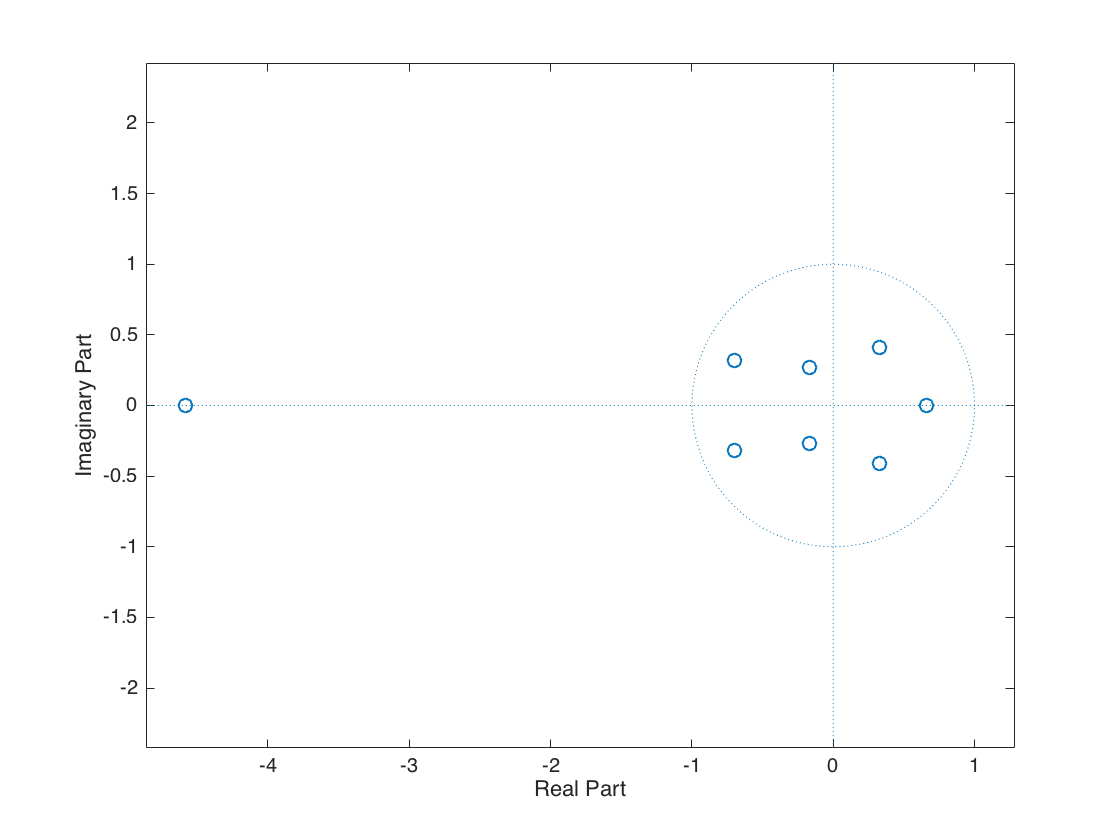
\includegraphics[angle=0,width=0.8\textwidth]{grafico_5_3_zplane.png}
     \captionof{figure}{Representação dos zeros da função de transferência do híbrido no plano Z}
     \label{fig:grafico_5_3_zplane}
\end{center}

Relacionando agora a resposta ao sinal de nível 1 da Figura \ref{fig:grafico_5_3} juntamente com o diagrama da Figura \ref{fig:grafico_5_3_zplane}, pode observar-se uma sobre-elevação acentuada, essencialmente devido aos zeros dentro do círculo unitário, do lado esquerdo do plano complexo. Seguidamente nota-se um seguimento ligeiramente oscilatório da referência, que se deve aos zeros dentro do círculo unitário, do lado direito do plano complexo, sendo o amortecimento devido em grande parte ao pólo presente no eixo real positivo. De notar também o facto de o valor da saída nunca ser inferior a 0 logo à partida, o que se deve à não-existência de zeros de fase não mínima.

De realçar também o ganho estático do filtro, que corresponde a fazer $z=1$ na função de transferência, o que dá um valor de $1.02$ V, que se pode observar no gráfico da figura \ref{fig:grafico_5_3}, uma vez que este corresponde a uma entrada do filtro unitária.

\chapter{Cancelador de Eco}

\section{Esquematização do sistema de teste}
Nos sistemas de comunicação convencionais, existe eco de linha gerado nos filtros híbridos do sistema, onde é feita a conversão do circuito a dois fios para o circuito a quatro fios. Em sistemas de transmissão de voz, o eco remoto assume particular importância pelo facto de que o orador é perturbado pelo eco da sua mensagem. Para comunicações a curta distância, o eco pode ser rápido o suficiente para que o cérebro humano não o detecte. Contudo, em comunicações a longa distância, o atraso pode ser significativo ao ponto de o emissor conseguir ouvir a sua voz repetidamente enquanto transmite a sua mensagem.\\
Nos sistemas de transmissão de dados, o eco mais relevante é o gerado no híbrido local, por poder ter uma amplitude largamente superior ao do sinal recebido do emissor remoto.\\

Nesta secção, será estudada e implementada uma solução para um cancelador de eco constituído por um filtro adaptativo a funcionar em modo de identificação recorrendo à estrutura FIR trasnversal adaptativa, representada na figura seguinte por um diagrama de blocos.

	 \begin{center}
     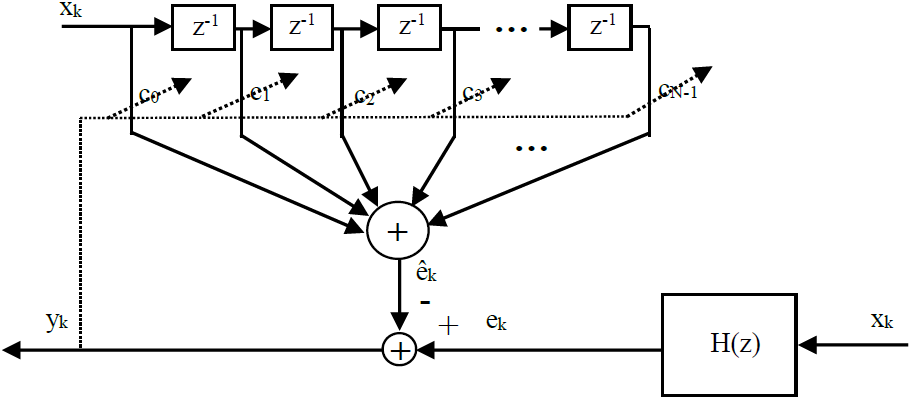
\includegraphics[angle=0,width=0.8\textwidth]{esquema.png}
     \captionof{figure}{ Diagrama de blocos do cancelador de eco local a implementar.}
     \label{fig:esquema}
     \end{center}
     
 Neste esquema, x$_k$ representa o sinal de dados de entrada que origina o eco, c$_i$ representa o coeficiente adaptativo da baixada $i$ do cancelador, y$_k$ representa o erro que serve, em retroacção, para adaptar os coeficientes do filtro, e$_k$ e ê$_k$ representam, respectivamente, o sinal de eco e a sua estimativa dada pelo cancelador e, por último, H$(z)$ representa a função de sistema do caminho do eco a identificar pelo filtro.\\
 
Para a adaptação dos coeficientes do filtro será utilizado o algoritmo LMS (Algoritmo do Gradiente Estocástico), segundo o qual a actualização a realizar em cada iteração (período de dados) se resume a:
\begin{equation} \label{eq:coef}
\textrm{c}_{i,k+1}=\textrm{c}_{i,k}+2\mu\, y_k\,\textrm{x}_{k-i}
\end{equation}

onde c$_{i,k}$ representa o valor do coeficiente da baixada $i$ na iteração $k$, $\mu$ é o passo de adaptação regulador da rapidez de convergência e da estabilidade, y$_k$ é o erro instantâneo e x$_{k-i}$ é a amostra do sinal originador de eco na baixada $i$ do filtro na iteração $k$.\\

Em série com o cancelador de eco será implementado um bloco de avaliação do eco, denominado ERLE (\emph{Echo Return Loss Enhancement}), definido como:
\begin{equation} \label{eq:contaerle}
ERLE=\dfrac{\textrm{E}[{e_k}^2]}{\textrm{E}[(e_k-ê_k)^2]}\Bigg|_{dB}
\end{equation}

\section{Implementação}

Tendo sido já descritos os blocos de geração de dados local e remoto, bem como o filtro híbrido, resta apenas apresentar a implementação realizada para o bloco de cálculo de ERLE, para o cancelador de eco e, por fim, para o sistema total que servirá de teste ao cancelador de eco.\\

\subsubsection{Cancelador de Eco}

Implementado em Simulink o esquema representado na figura \ref{fig:esquema}, obtém-se o seguinte diagrama:
\begin{center}
     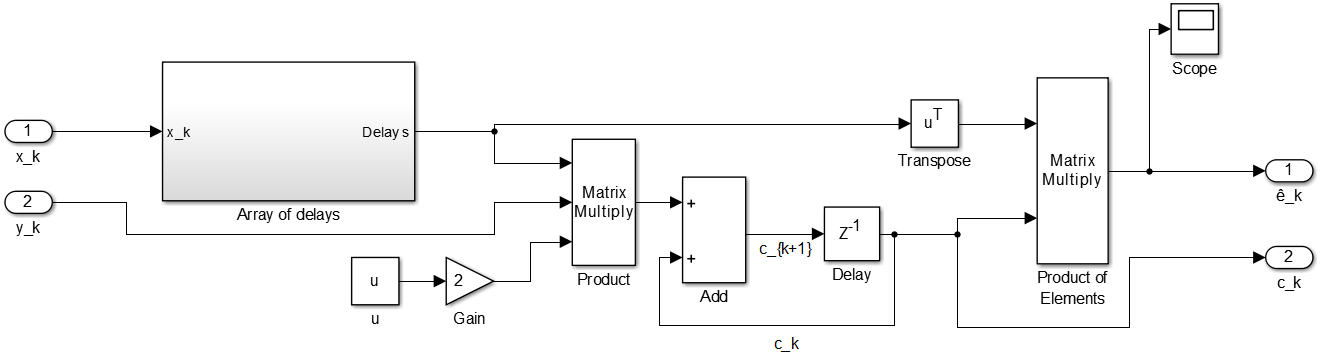
\includegraphics[angle=0,width=1\textwidth]{cancelador.png}
     \captionof{figure}{ Diagrama de blocos em Simulink do cancelador de eco implementado.}
     \label{fig:cancelador}
     \end{center}

onde o bloco \emph{Array of delays} é responsável pela criação das baixadas do filtro a partir do sinal de dados e pela sua vectorização.

\begin{center}
     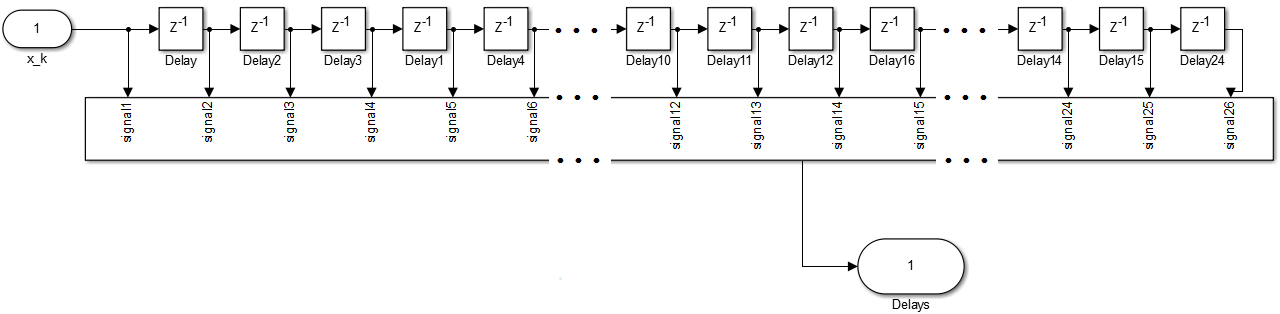
\includegraphics[angle=0,width=1.1\textwidth]{delays.png}
     \captionof{figure}{ Diagrama de blocos em Simulink das baixadas do filtro FIR transversal.}
     \label{fig:delays}
     \end{center}

Este sub-sistema coloca cada baixada dos dados num vector coluna, fazendo corresponder a cada linha o índice da baixada. Como todas as restantes grandezas no segundo termo do membro direito da equação \ref{eq:coef} são escalares, os coeficientes serão obtidos também num vector coluna. Desta forma, a obtenção de ê$_k$ fica reduzida à elegante operação matricial
\begin{equation}
ê_k=\begin{bmatrix}
           \textrm{x}_{k-0} \\
           \textrm{x}_{k-1} \\
           \vdots \\           
           \textrm{x}_{k-25} \\
           \end{bmatrix}^T \times
           \begin{bmatrix}
           \textrm{c}_{0,k} \\
           \textrm{c}_{1,k} \\
           \vdots \\           
           \textrm{c}_{25,k} \\
           \end{bmatrix}           
\end{equation}

onde o vector coluna com as baixadas com dados de entrada é transposto de forma a que a multiplicação resulte no escalar pretendido.

\subsubsection{ERLE}

A implementação da equação \ref{eq:contaerle} resultou no seguinte diagrama:

\begin{center}
     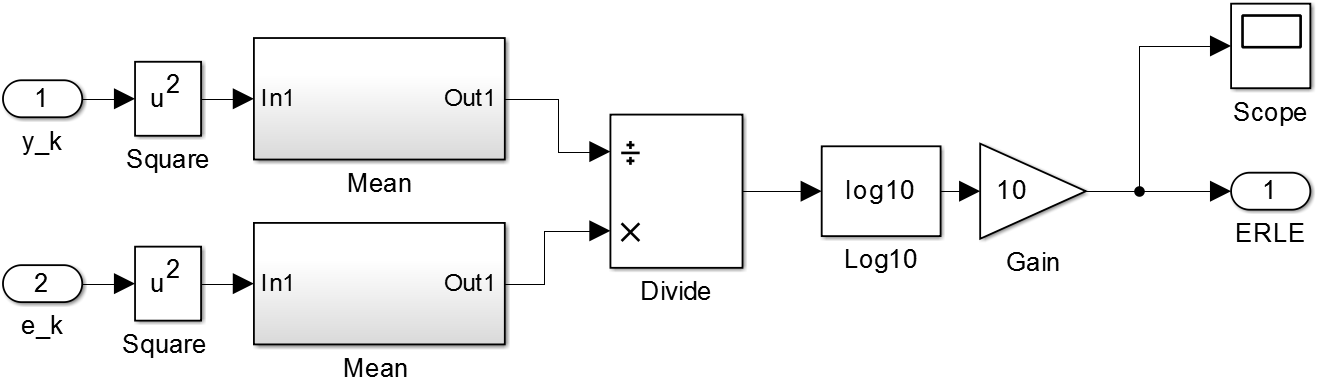
\includegraphics[angle=0,width=1\textwidth]{erle.png}
     \captionof{figure}{ Diagrama de blocos em Simulink do bloco de cálculo de ERLE.}
     \label{fig:erle}
     \end{center}
     
Interessa mencionar a função gerada para a obtenção da média instantânea (\emph{Mean}). Na figura seguinte encontra-se a sua implementação.

\begin{center}
     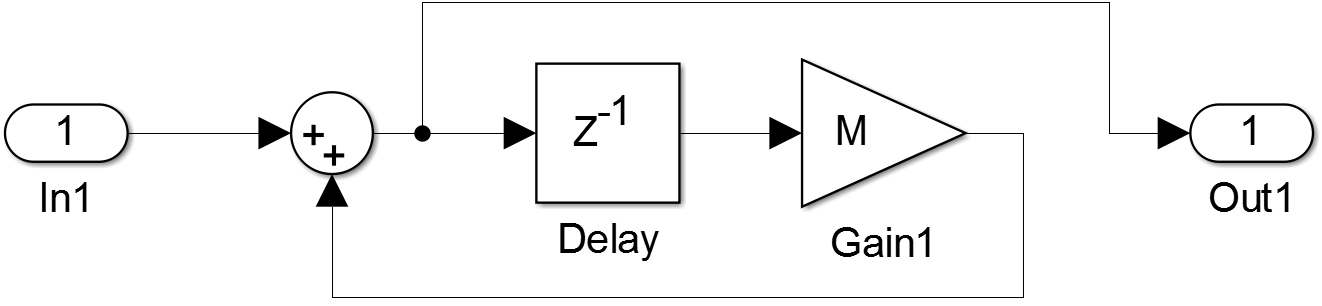
\includegraphics[angle=0,width=0.8\textwidth]{mean.png}
     \captionof{figure}{ Diagrama de blocos em Simulink do bloco de cálculo da média instantânea.}
     \label{fig:mean}
     \end{center}

A função de transferência deste bloco é dada por:

\begin{equation}
\dfrac{Out1(z)}{In1(z)}=\dfrac{z+M}{z}
\end{equation}

Fazendo M=$0.95$ e para uma frequência de amostra de 1 segundo (frequência dos dados), obteve-se o seguinte diagrama de bode de magnitude:
\begin{center}
     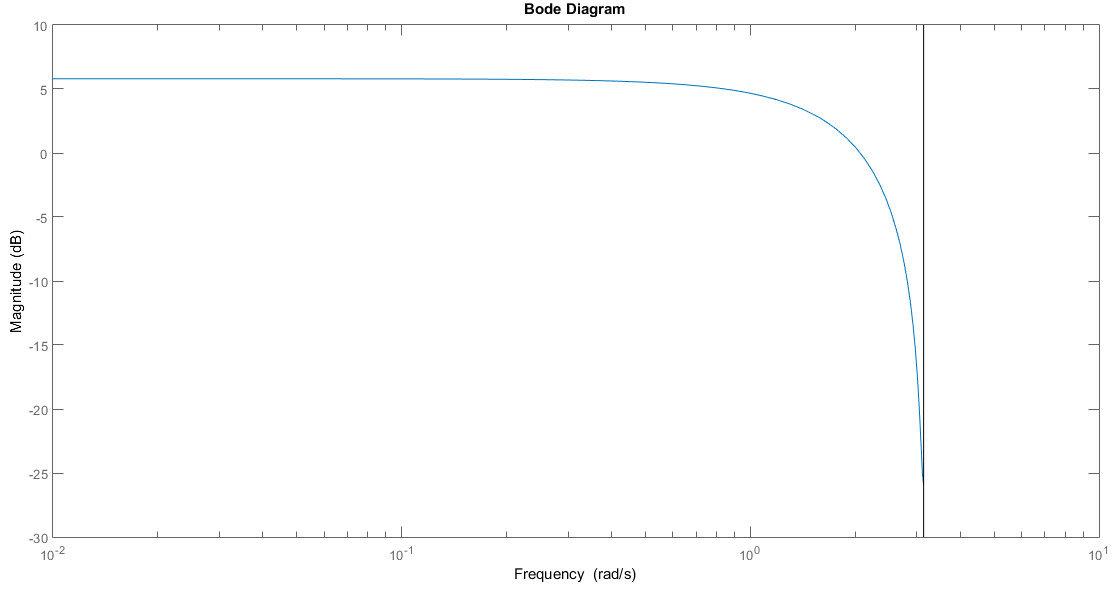
\includegraphics[angle=0,width=0.8\textwidth]{meanmag.png}
     \captionof{figure}{ Diagrama de bode de magnitude da função de transferência de \emph{Mean}.}
     \label{fig:meanmag}
     \end{center}

Ou seja, podemos constatar que a partir de aproximadamente 2 radianos por segundo a entrada já é bastante atenuada, o que nos leva a concluir que este bloco funciona como um filtro passa-baixo com uma frequência de corte extremamente baixa. A utilização deste filtro de primeira ordem como operador ``média'' é eficaz porque com estas características permite obter apenas à saída a componente contínua do sinal de entrada, ou seja, a média do sinal.


\section{Teste e Análise}

Para o teste do cancelador de eco, implementa-se em paralelo com este um filtro de quarta ordem H$(z)$ com todas as baixadas com coeficientes nulos à excepção da última que tem coeficiente unitário. Quando o circuito convergir, isto é, quando o erro y$_k$ tender para zero, espera-se que o cancelador de eco identifique correctamente o filtro H$(z)$, ou seja, os coeficientes dos dois filtros são iguais nas baixadas comuns. Para os coeficientes das baixadas superiores a 4, espera-se que sejam nulos no cancelador de eco.\\

O diagrama a simular neste teste corresponde então ao esquema da seguinte figura.

\begin{center}
     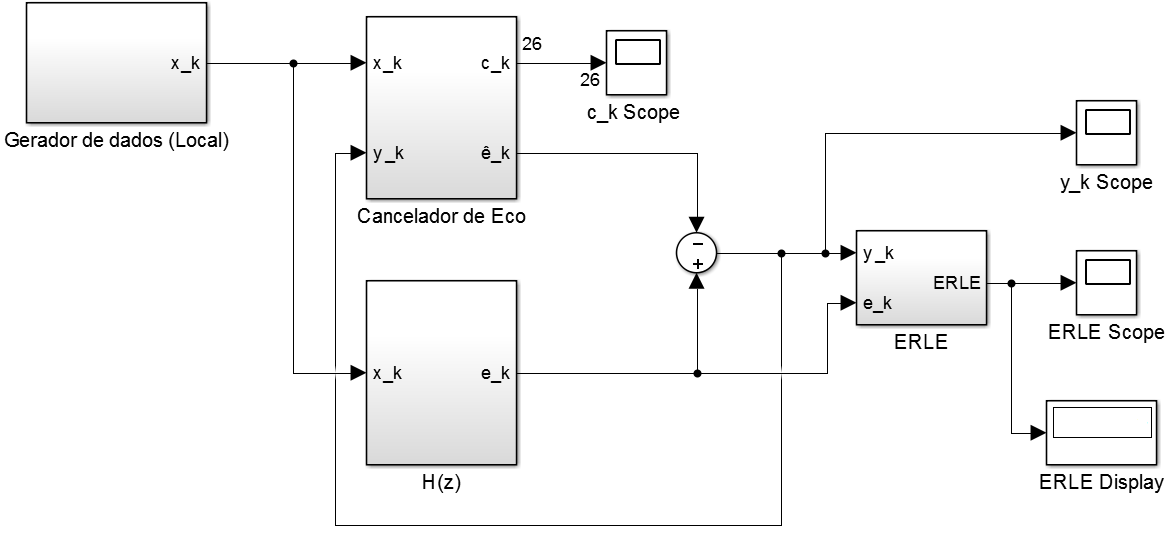
\includegraphics[angle=0,width=0.9\textwidth]{testecancelador.png}
     \captionof{figure}{ Circuito de teste do cancelador de eco.}
     \label{fig:testecancelador}
     \end{center}

Utilizando na simulação uma frequência de amostragem unitária (igual ao ritmo de transmissão de dados) e um passo de adaptação $\mu=$0.03, obteve-se o seguinte gráfico à saída do bloco ERLE:

\begin{center}
     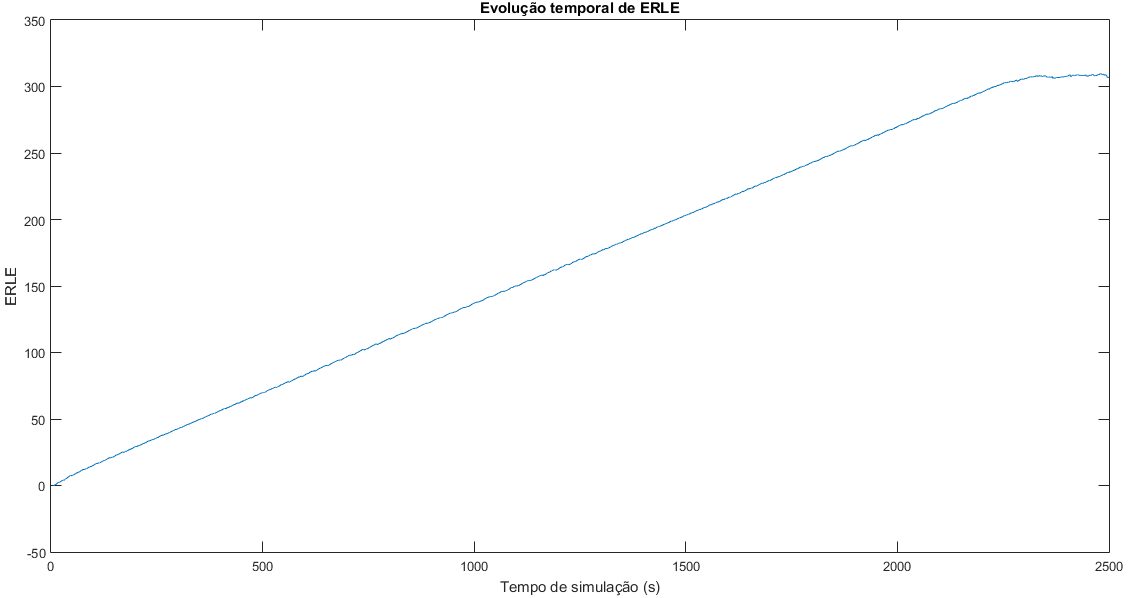
\includegraphics[angle=0,width=0.9\textwidth]{testecanceladorERLE.png}
     \captionof{figure}{ Parâmetro ERLE em função do tempo no teste do cancelador de eco}
     \label{fig:testecanceladorERLE}
     \end{center}

O facto de ERLE estabilizar para o passo de adaptação escolhido prova que o cancelador de eco está a funcionar correctamente, ou seja, a estimação do eco iguala eventualmente o eco real do sistema de transmissão, anulando o erro. Adicionalmente, podemos observar a correcta identificação do filtro de quarta ordem analisando a evolução temporal dos coeficientes do cancelador.

\begin{center}
     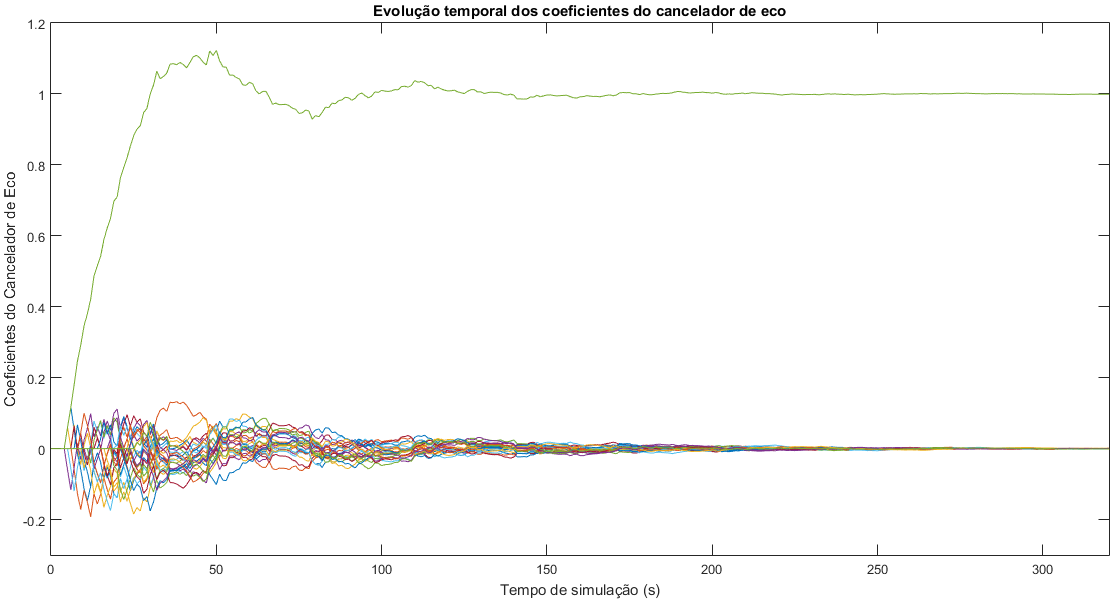
\includegraphics[angle=0,width=1\textwidth]{testecanceladorCoef.png}
     \captionof{figure}{ Coeficientes adaptativos em função do tempo no teste do cancelador de eco}
     \label{fig:testecanceladorCoef}
     \end{center}

Como é possível observar, os coeficientes estabilizam num tempo muito inferior ao necessário para a estabilização de ERLE para o valor de $\mu$ escolhido e em regime estacionário apresentam os valores que esperávamos obter: todos os coeficientes são nulos à excepção do da baixada 4 que é a unidade. Na tabela seguinte encontram-se os valores exactos e aproximados dos valores dos coeficientes na última iteração da simulação realizada, largos segundos após a estabilização dos mesmos.

\begin{table}[H]
  \centering
    \begin{tabular}{|ccc|}
    \hline
    \textbf{Baixada} & \textbf{Valor Estabilizado} & \textbf{Valor Aproximado} \\
    \hline
    0     & 5,84346620219036e-17 & 0 \\
    1     & 1,76751392447828e-17 & 0 \\
    2     & 1,65265133686427e-16 & 0 \\
    3     & -7,49553910329146e-17 & 0 \\
    4     & 1     & 1 \\
    5     & -5,96745511362410e-17 & 0 \\
    6     & -4,44438335186570e-17 & 0 \\
    7     & -1,44060255594206e-16 & 0 \\
    8     & -9,13444252608803e-18 & 0 \\
    9     & -4,89371590020595e-17 & 0 \\
    10    & -3,06580780917038e-17 & 0 \\
    11    & 1,22820592389783e-18 & 0 \\
    12    & -5,55856328768580e-17 & 0 \\
    13    & 1,41629278738278e-16 & 0 \\
    14    & -8,01886251849398e-17 & 0 \\
    15    & 5,91975627211735e-17 & 0 \\
    16    & -2,20505787446950e-17 & 0 \\
    17    & 1,00464454030339e-16 & 0 \\
    18    & 1,02684281813918e-16 & 0 \\
    19    & 9,22976684109320e-17 & 0 \\
    20    & -1,31873919970781e-16 & 0 \\
    21    & 3,74441232299027e-17 & 0 \\
    22    & 1,59308979488315e-16 & 0 \\
    23    & 5,70847401452762e-17 & 0 \\
    24    & 4,06539484403783e-17 & 0 \\
    25    & -6,56421426138642e-17 & 0 \\
    \hline
    \end{tabular}\caption{Valores estacionários dos coeficientes do cancelador de eco}
  \label{tab:addlabel}%
\end{table}%





\chapter{Sistema Total}
\section{Implementação}

Construíu-se o circuito total para a simulação do cancelamento de eco num sistema de transmissão de dados, combinando os blocos descritos anteriormente segundo a configuração representada pela figura \ref{fig:total}.

\begin{center}
     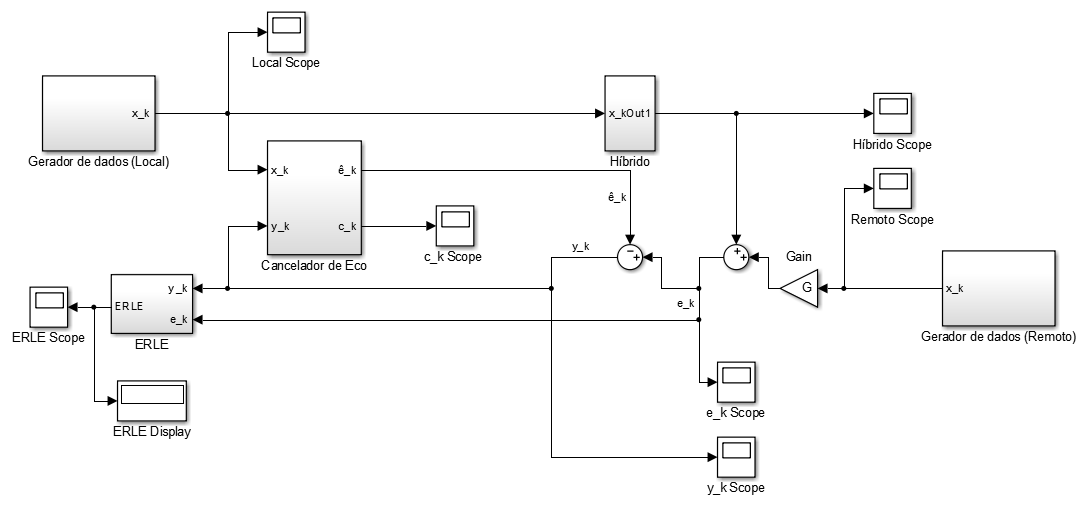
\includegraphics[angle=0,width=1.1\textwidth]{STotal.png}
     \captionof{figure}{ Circuito total de simulação do cancelamento de eco num sistema de transmissão de dados.}
     \label{fig:total}
     \end{center}


 O circuito completo pode ser interpretado como a conciliação de 4 diferentes secções:

\begin{itemize}
\item  \textbf{Gerador de eco proveniente do emissor local} - secção constituída pelos blocos \textit{Gerador de Dados (Local)} e \textit{Híbrido}. O primeiro é responsável pelo fornecimento de dados pseudo-aleatórios e o segundo, tem o papel de filtro, simulando o eco originado pela passagem de 4 fios (emissor/receptor) para 2 fios (linha de transmissão).

\item \textbf{Gerador de ruído proveniente do emissor remoto} - secção constituída pelos blocos \textit{Gerador de Dados (Remoto)} e \textit{Ganho}. De forma análoga à secção anterior, o primeiro bloco é responsável pelo fornecimento de dados pseudo-aleatórios, sendo que o segundo, o bloco de ganho, $G$, permite atenuar o sinal emitido pelo emissor remoto, simulando ruído.

\item \textbf{Cancelamento do eco/ruído no sistema} - secção constituída pelo bloco \textit{Cancelador de Eco}. Este corresponde a um filtro adaptativo, que permite estimar a soma eco+ruído do sistema (soma dos sinais de saída das secções anteriores). Apresenta como sinal de saída a estimativa, $ê_k$, do valor real, $e_k$. O bloco subtracção  $e_k-ê_k$ implementa o cancelamento do eco.

\item \textbf{Avaliador do cancelamento de eco} - secção constituída pelo bloco \textit{ERLE}, que permite obter o parâmetro de eficiência no cancelamento do eco em $dB$ (um bom cancelamento implica $ERLE\gg 1$).
\end{itemize}





\section{Teste e Análise}

\subsection{Teste do sistema sem ruído}



\large\underline{{\textit{\textbf{Implementação do passo de adaptação $\mu=0.03$}}}}\\
\par
Pretendeu-se analisar o sistema total para o caso em que $G=0$, isto é, sem ruído. 

Começou-se por implementar um passo de adaptação $\mu=0.03$ e tempo de aquisição, $T=5000s$. Obtiveram-se os gráficos  das evoluções no tempo, do $ERLE$ (figura \ref{fig:SRu003}) e dos valores dos coeficientes do \textit{Cancelador de Eco}, $c_k$ (figura \ref{fig:SRu003t}).


\begin{center}
     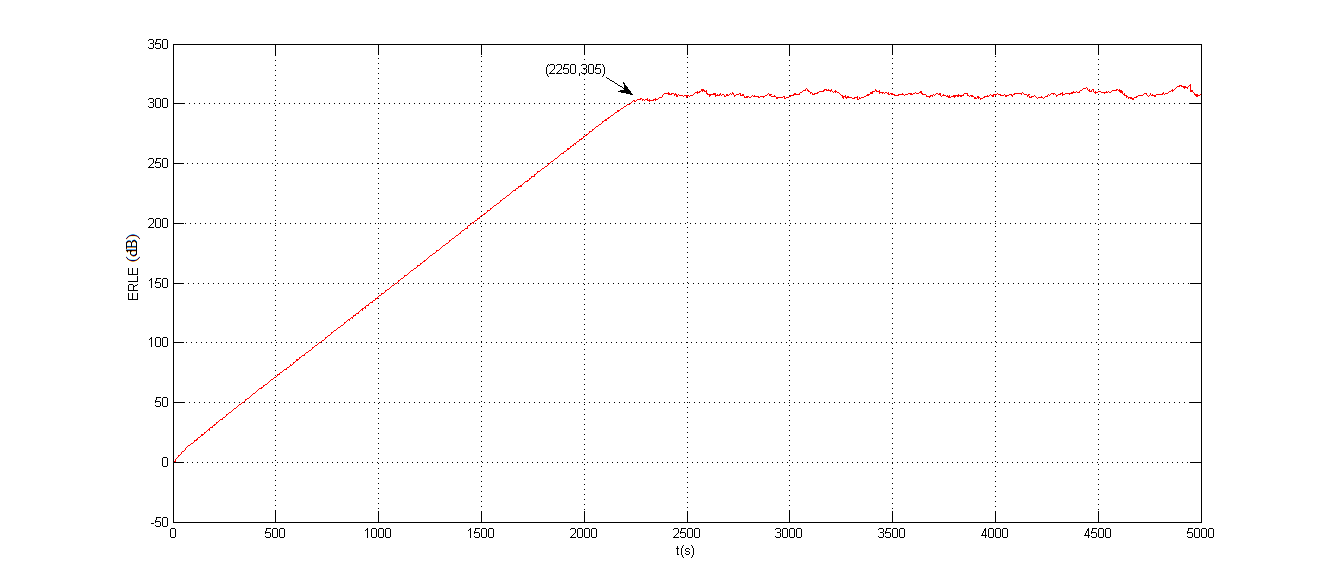
\includegraphics[angle=0,width=1\textwidth]{SRu003.png}
     \captionof{figure}{ Gráfico parâmetro de eficiência, $ERLE$ $(dB)$, em função do tempo, $t(s)$, para $\mu=0.03$ e $T=5000s$.}
     \label{fig:SRu003}
     \end{center}
´

\begin{center}
     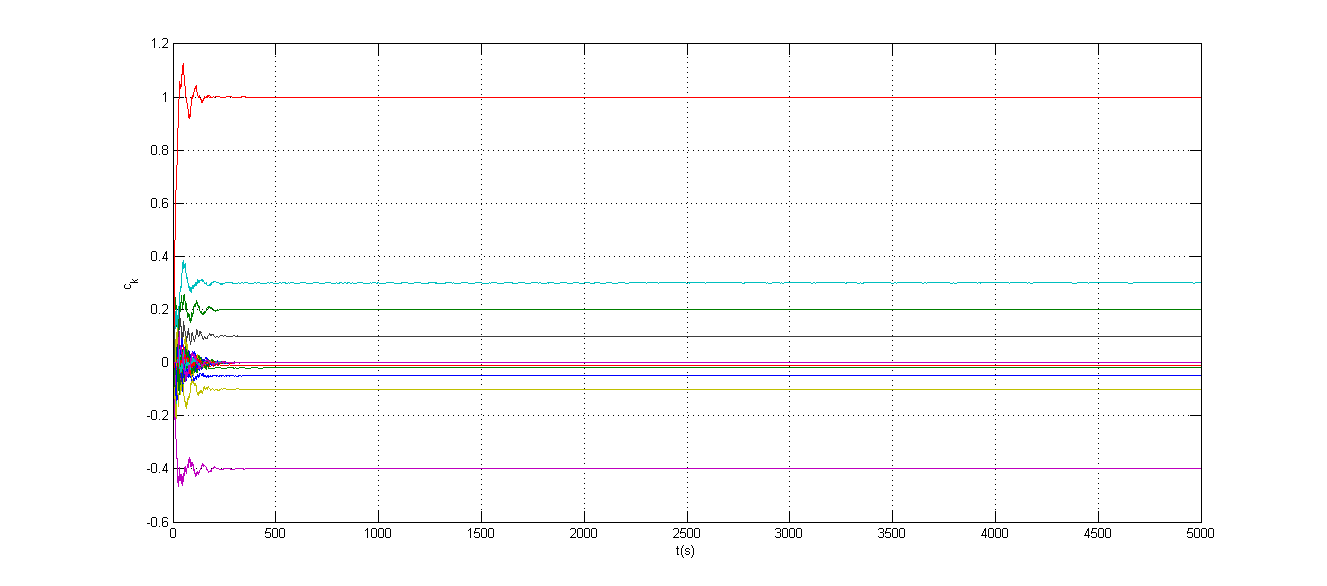
\includegraphics[angle=0,width=1\textwidth]{SRu003t.png}
     \captionof{figure}{ Gráfico coeficientes $c_k$ em função do tempo, $t(s)$, para $\mu=0.03$ e $T=5000s$.}
     \label{fig:SRu003t}
     \end{center}

Analisando o gráfico da figura \ref{fig:SRu003}, podemos verificar, um aumento monótono e uniforme do valor do $ERLE$ até um instante de estagnação (convergência), sendo este:

$$t_{0}\approx2250s$$

Obteve-se o valor do $ERLE$ nesse instante, $ERLE_{0}=ERLE(t_{0})=305dB$. Portanto, no regime transitório, $t\in[0,t_{0}]$, a taxa de variação temporal do $ERLE$ foi:

$$\frac{d}{dt}\left(ERLE\right)\approx{\frac{ERLE_{0}}{t_{0}}}\approx0.136dB/s$$   

 Para $t>t_{0}$ verificaram-se pequenas oscilações em torno do ponto de equilíbrio (média dos valores do ERLE no regime estacionário):
 $$\langle{ERLE}_{st}\rangle=307.73dB\gg1$$
 
 o que corresponde a um cancelamento bastante significativo do eco no sistema. O valor médio relativo das oscilações em torno de $\langle{ERLE}_{st}\rangle$ foi:
 $$\langle O(ERLE_{st}) \rangle_r= 0.57 \%$$

\vspace{15pt}
 
 
\begin{center}
* * *
\end{center}

\underline{\textbf{Nota}}: Expressão usada para o cálculo do valor médio relativo das oscilações: $$\langle O(ERLE_{st}) \rangle_r=\frac{\langle |ERLE_{st}-\langle ERLE_{st} \rangle| \rangle}{\langle ERLE_{st} \rangle}$$ 

\begin{center}
* * *
\end{center}

\vspace{15pt}
 


Relativamente ao gráfico da figura \ref{fig:SRu003t}, podemos constatar um regime oscilatório dos valores dos coeficientes $c_k$, do instante inicial $t=0s$ até ao instante de convergência $t_{0,c}\approx 250s$, tornando-se estes constantes para $t>t_{0,c}$ (regime de estacionariedade).\\
\par

\large\underline{{\textit{\textbf{Implementação de passo de adaptação 10 vezes menor ($\mu=0.003$)}}}}\\
\par

De seguida alterou-se o valor do passo adaptação para um valor 10 vezes menor que o anterior, isto é, $\mu=0.003$, tendo-se obtido os gráficos \ref{fig:SRu0003} e \ref{fig:SRu0003t}.


\begin{center}
     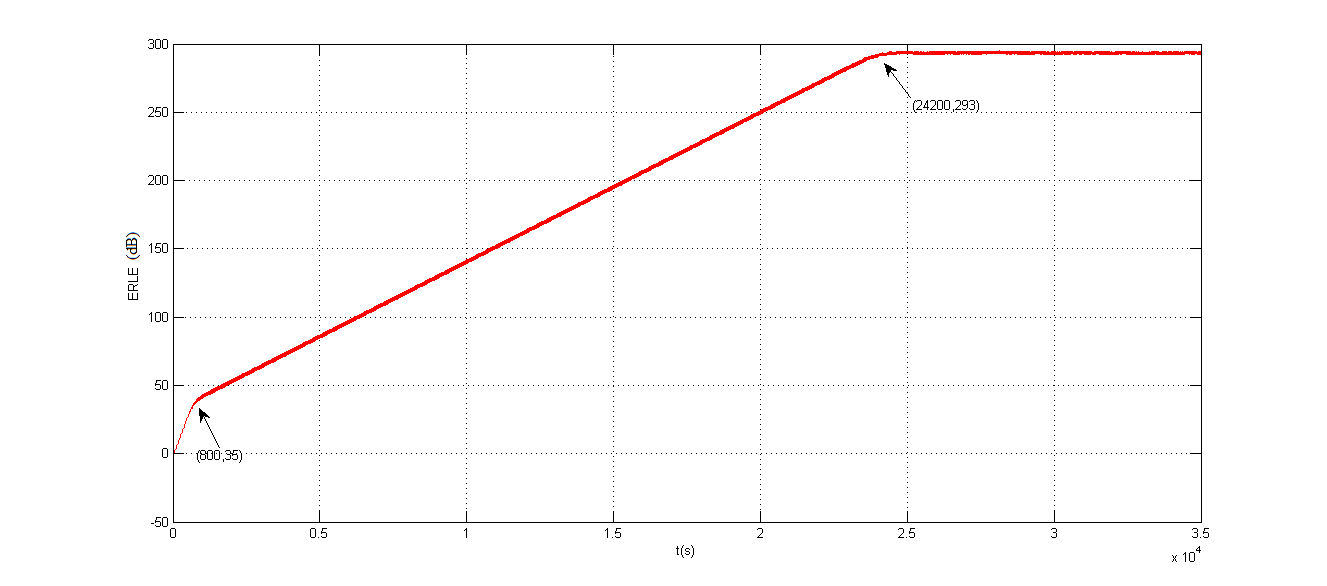
\includegraphics[angle=0,width=1\textwidth]{SRu0003.png}
     \captionof{figure}{ Gráfico parâmetro de eficiência $ERLE$ ($dB$) em função do tempo, $t(s)$, para $\mu=0.003$ e $T=35000s$.}
     \label{fig:SRu0003}
     \end{center}


\begin{center}
     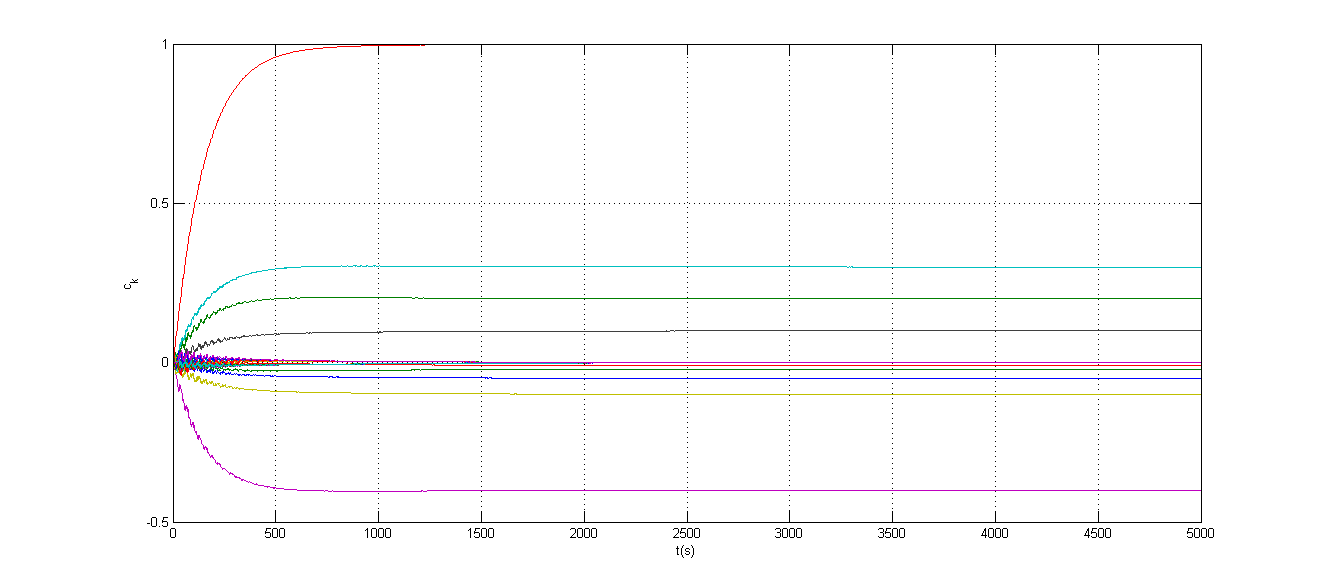
\includegraphics[angle=0,width=1\textwidth]{SRu0003t.png}
     \captionof{figure}{ Gráfico coeficientes $c_k$ em função do tempo, $t(s)$, para $\mu=0.003$ e $T=35000s$. (Restringíu-se o $range$ no eixo dos $x$ para $[0,5000]$, de forma que a que o regime transitório dos coeficientes $c_k$ fosse mais fácil de visualizar). }
     \label{fig:SRu0003t}
     \end{center}

Analisando o gráficos  \ref{fig:SRu0003}, podemos identificar três regimes de comportamento da eficiência $ERLE$, com o tempo. 

Para $t\in[0,800] s$ (considere-se $t_{p}=800s$) tem-se um regime transitório, cuja taxa de variação é maior, sendo $ERLE_p=ERLE(t_p)=35dB$. Obteve-se:

$$\left(\frac{d}{dt}\left(ERLE\right)\right)_{1}\approx{\frac{ERLE_{p}}{t_{p}}}\approx0.044dB/s$$ 

o que corresponde a um valor 3.09 vezes menor que o obtido para $\mu=0.03$.\\
\par
Para $t\in[0,24200] s$ (considere-se $t_{0}=24200s$) tem-se um regime transitório de taxa de variação menor. O $ERLE$ estagna no instante:

$$t_{0}\approx24200s$$ sendo $ERLE_{0}=ERLE(t_{0})\approx293dB$. Obteve-se assim para este regime:


$$\left(\frac{d}{dt}\left(ERLE\right)\right)_{2}\approx{\frac{ERLE_{0}-ERLE_p}{t_{0}-t_p}}\approx0.011dB/s$$ 

Esta taxa de variação é 4 vezes menor que $\left(\frac{d}{dt}\left(ERLE\right)\right)_{1}$ e 12.36 vezes menor que a taxa de variação para o caso $\mu=0.03$. O tempo necessário para optimizar a estimativa do eco pelo \textit{Cancelador de Eco}, é portanto maior:

$$t_{0}\bigg{|}_{\mu=0.003}=10.76\hspace{3pt}t_{0}\bigg{|}_{\mu=0.03}$$

Isto significa que são necessárias 10.76 vezes mais iterações para $\mu=0.003$ para se atingir a convergência da estimativa do eco+ruído, que para o caso $\mu=0.03$.

É importante ainda referir que o tempo de convergência para $\mu=0.03$ foi suficientemente reduzido para não se notarem 2 diferentes regimes de transição do $ERLE$, tal como se constatou para o caso de  $\mu=0.003$.\\
\par No regime estacionário, $t\in[24200,35000]$, obteve-se:

$$\langle ERLE_{st}\rangle=293.44dB\gg1$$ portanto, um valor bastante satisfatório e próximo do obtido para $\mu=0.03$, isto é, com um desvio de $4.64\%$. O valor médio relativo das oscilações neste regime foi: $$\langle O(ERLE_{st})_r \rangle=0.14\%$$ ou seja 4.23 vezes menor que o obtido para $\mu=0.03$. É portanto correcto afirmar que o processo para $\mu=0.003$ é mais estável (no sentido das perturbações) que para $\mu=0.03$. \\
\par
Relativamente ao gráfico da figura \ref{fig:SRu0003t}, pode-se dizer que o instante de convergência das constantes $c_k$ foi na gama $t_{0,c}\in[600,1000]s$, também superior ao obtido para $\mu=0.03$. \\
\par

\large\underline{{\textit{\textbf{Determinação de $\mu_{máx}$ para o qual se tem um processo estável}}}}\\
\par

Pretendeu-se de seguida, determinar o valor máximo do passo $\mu$ para o qual se continua a obter um processo estável. Um processo estável deverá realizar a função que se pretende, isto é, o cancelamento do eco ($ERLE>0dB$), e com reduzidas perturbações. Construíu-se a tabela \ref{tab:mu}.


\begin{table}[h]
\centering
\begin{tabular}{ || c | c | c | c | c | c || }
\hline
	$\mu$ & $t_0$(s) & $T$(s) & $\frac{\Delta ERLE}{\Delta t}$ ($dB/s$) & $\langle ERLE_{st}\rangle (dB)$ & $\langle O(ERLE_{st})\rangle_r$ (\%) \\ \hline  \hline
	0.0030 & 24200 & 35000 & 0.012 & 293.437 & 0.135   \\ \hline
	0.0100 & 6000 & 8000 & 0.051 & 303.908 & 0.258   \\ \hline
	0.0150 & 3500 & 5000 & 0.090 & 314.307 & 0.520   \\ \hline
	0.0200 & 1935 & 3500 & 0.160 & 312.917 & 0.506   \\ \hline
	0.0225 & 1450 & 5000 & 0.215 & 315.665 & 0.833  \\ \hline
	\multirow{2}{*}{0.0250} & 1500 & \multirow{2}{*}{5000} & 0.210 & 313.342 & 0.750   \\ \hhline{~-~---}
	 & 3950 &  & 0.086 & 340.424 & 0.414   \\ \hline
	\multirow{2}{*}{0.0275} & 1660 & \multirow{2}{*}{5000} & 0.187 & 310.546 & 0.658   \\ \hhline{~-~---}
	 & 3900 &  & 0.086 & 335.563 & 0.511  \\ \hline
	0.0300 & 2250 & 5000 & 0.136 & 307.730 & 0.573  \\ \hline
	0.0325 & 3450 & 5000 & 0.088 & 304.040 & 0.449   \\ \hline
	0.0350 & 6300 & 10000 & 0.048 & 301.398& 0.367   \\ \hline
	0.0375 & 23200 & 30000 & 0.013 & 294.612 & 1.442   \\ \hline
	0.0380 & 50000 & 100000 & 0.006 & 290.345& 0.424   \\ \hline
	0.03846 & --- & 100000 & --- & 14.998 & 4.415  \  \\ \hline
	0.0390 & --- & 100000 & -0.019 & --- & ---  \  \\ \hline
\end{tabular}

\caption{Valores obtidos do tempo de convergência, $t_{0}$, declive da reta que une o ponto $(t_0,ERLE_{0})$ à origem, $\frac{\Delta ERLE}{\Delta t}$, $ERLE$ médio, $\langle ERLE_{st}\rangle$, e oscilações médias do ERLE, $\langle O(ERLE_{st})\rangle$, no regime de estacionariedade, para diferentes passos $\mu$.\label{tab:mu}}

\end{table}

A tabela \ref{tab:mu} apresenta 4 casos particulares para os valores de $\mu=0.0250$, 0.0275, 0.03846 e 0.0390, que devem de ser explicitados. \\
\par
\large\underline{{\textit{{Análise para os passos de adaptação $\mu=0.0250$ e $\mu=0.0275$}}}}\\
\par
Para $\mu=0.0250$ e $\mu=0.0275$ obtiveram-se 4 regimes de comportamento do $ERLE$ com o tempo: 2 regimes transitórios e 2 regimes de estacionariedade, tal como demonstram os gráficos $\ref{fig:mu00250}$ e $\ref{fig:mu00275}$.

\begin{center}
     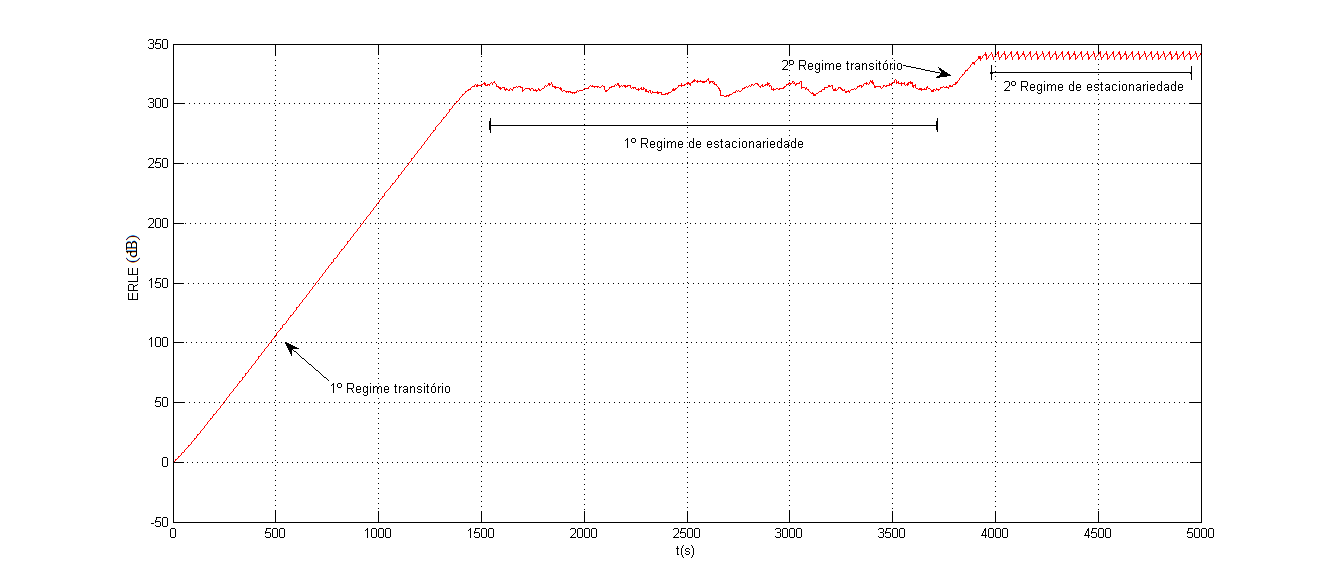
\includegraphics[angle=0,width=1\textwidth]{mu00250.png}
     \captionof{figure}{ Gráfico parâmetro de eficiência $ERLE$ ($dB$) em função do tempo, $t(s)$, para $\mu=0.0250$ e $T=5000s$.}
     \label{fig:mu00250}
       \end{center}
  

\begin{center}
     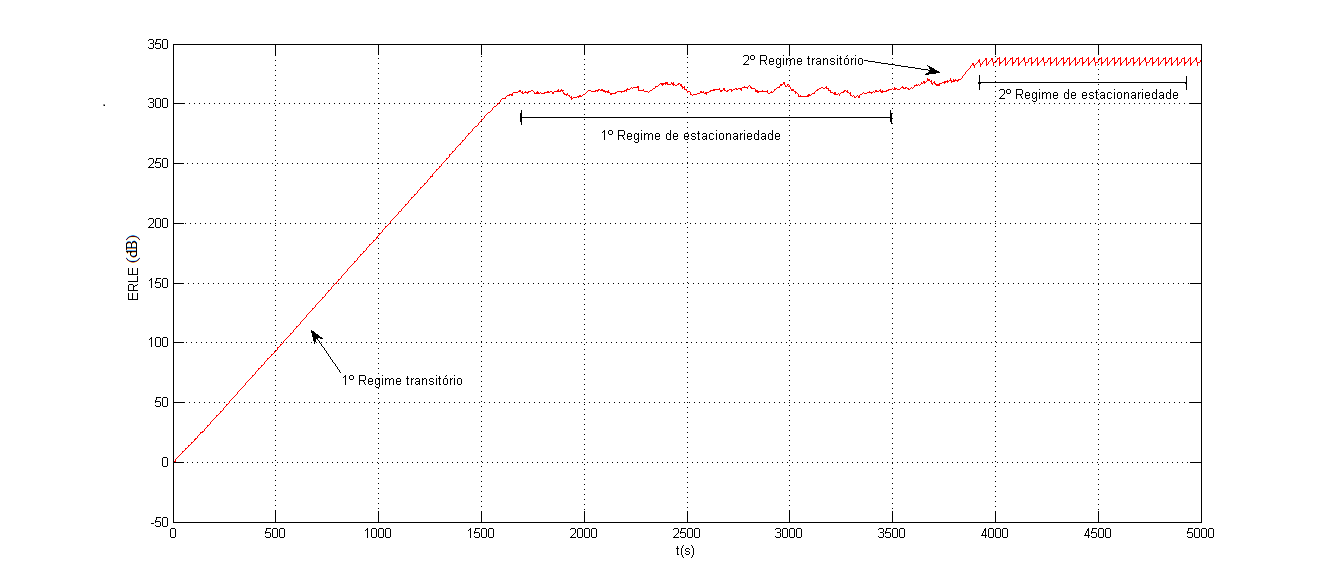
\includegraphics[angle=0,width=1\textwidth]{mu00275.png}
     \captionof{figure}{ Gráfico parâmetro de eficiência $ERLE$ ($dB$) em função do tempo, $t(s)$, para $\mu=0.0275$ e $T=5000s$.}
     \label{fig:mu00275}
     \end{center}

Devido a estas características dos gráficos decidiu-se considerar na tabela \ref{tab:mu} o declive da reta que une o ponto $(t_0,ERLE_{0})$ à origem $O$, $\frac{\Delta ERLE}{\Delta t}$, em vez da taxa de variação temporal do $ERLE$ no regime transitório, $\frac{d}{dt}\left(ERLE\right)$, já que o primeiro permite estabelecer uma relação imediata ${ERLE_0}_k/t_{0_k}$, isto é, o rácio entre o valor do $ERLE$ no instante da $k-ésima$ convergência, $t_{0_k}$, e o tempo necessário para este valor ser atingido, o próprio $t_{0_k}$. É mais interessante avaliar a transição total do $ERLE$  até aos pontos de convergência, do que avaliar apenas os regimes transitórios deste.  \\

\par É ainda importante referir que, na tabela \ref{tab:mu}, $\frac{\Delta ERLE}{\Delta t}$ coincide com $\frac{d}{dt}\left(ERLE\right)$ para todos os outros valores de $\mu$, à excepção de $\mu=0.0030$, que apresenta duas zonas de transição consecutivas (existe apenas um instante te estagnação $t_0$).\\
\par
\large\underline{{\textit{Análise para o passo de adaptação $\mu=0.03846$}}}\\
\par
\textbf{O passo crítico para a estabilidade do processo, corresponde a $\mu_c=0.03846$ (=$\mu_{máx}$)}. Este, foi determinado varrendo os valores de $\mu$ numa região de comportamento limite, tal que $\mu<\mu_c$ implicava estabilidade do processo e $\mu>\mu_c$ implicava instabilidade do processo. O gráfico $ERLE$ em função do tempo, $t$, obtido para $\mu=0.03846$ encontra-se na figura \ref{fig:mu003846}.

\begin{center}
     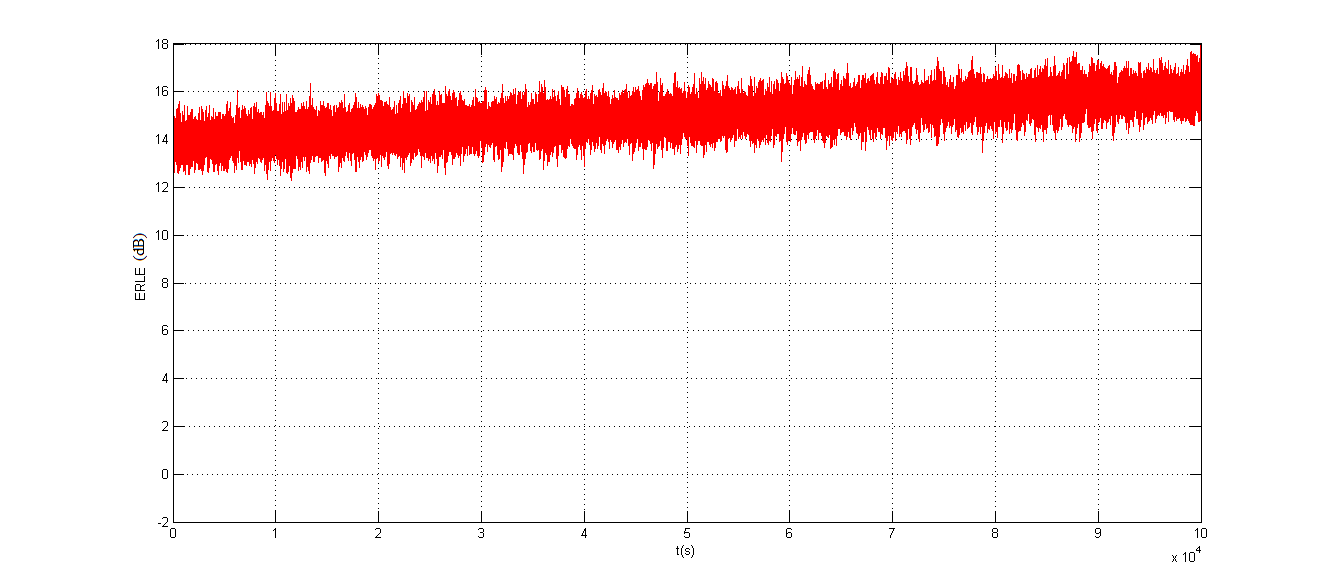
\includegraphics[angle=0,width=1\textwidth]{mu003846.png}
     \captionof{figure}{ Gráfico parâmetro de eficiência $ERLE$ ($dB$) em função do tempo, $t(s)$, para $\mu=0.03846$ e $T=100000s$.}
     \label{fig:mu003846}
     \end{center}
     
Para $\mu=0.03846$, o $ERLE$ oscila em torna de um ponto de equilíbrio sensivelmente constante, $\langle ERLE \rangle=14.998dB$. As perturbações foram bastante significativas  já que $\langle O(ERLE)\rangle_r=4.415\%$, o valor mais alto apresentado na tabela \ref{tab:mu}.\\
\par 
Para  $\mu<\mu_c$ obtiveram-se tempos de convergência, $t_0$, muito grandes tal como revela a tabela \ref{tab:mu}, $\left(t_{0_{(\mu=0.0380)}}\approx50000s\right)$.
Para $\mu>\mu_c$, o $ERLE$ assumia valores negativos, diminuindo monotonamente e uniformemente. \\
\par
\large\underline{{\textit{Análise para o passo de adaptação $\mu=0.0390$}}}\\
\par

Tal como foi registado na tabela \ref{tab:mu}, para $\mu=0.0390$ obteve-se $\frac{d}{dt}\left(ERLE\right)=-0.019dB/s$, sendo que o gráfico $ERLE$ em função do tempo, $t$, não apresenta nenhum ponto de convergência (figura \ref{fig:mu00390}). 

\begin{center}
     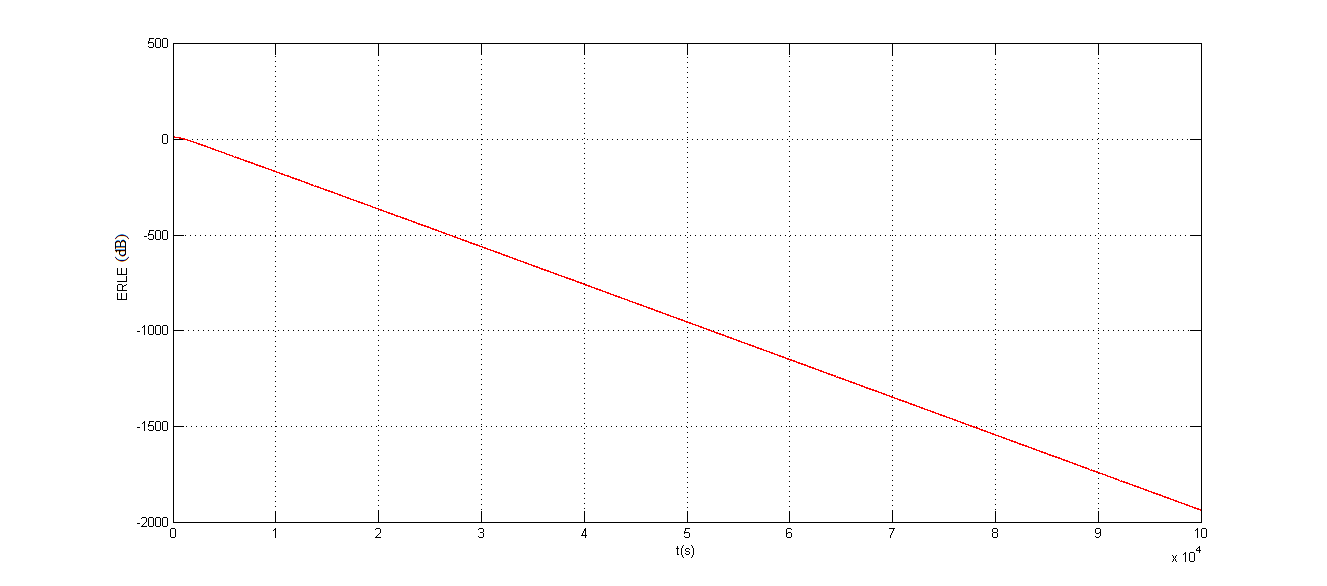
\includegraphics[angle=0,width=1\textwidth]{mu00390.png}
     \captionof{figure}{ Gráfico parâmetro de eficiência $ERLE$ ($dB$) em função do tempo, $t(s)$, para $\mu=0.0390$ e $T=100000s$.}
     \label{fig:mu00390}
     \end{center}
     
     
\large\underline{{\textit{Análise da variação de $t_0$, $\frac{\Delta ERLE}{\Delta t}$, $\langle ERLE_{st}\rangle$ e $\langle O(ERLE_{st})\rangle_r$ com $\mu$}}}\\
\par


Com os dados da tabela \ref{tab:mu} construíram-se os graficos $t_0$(s), $\frac{\Delta ERLE}{\Delta t}$($dB/s$), $\langle ERLE_{st}\rangle$ ($dB$) e $\langle O(ERLE_{st})\rangle_r$ ($\%$) em função do passo de adaptação, $\mu$. Estes apresentam-se nas figuras \ref{fig:t0}, \ref{fig:declive}, \ref{fig:med} e \ref{fig:osc}.

\begin{center}
     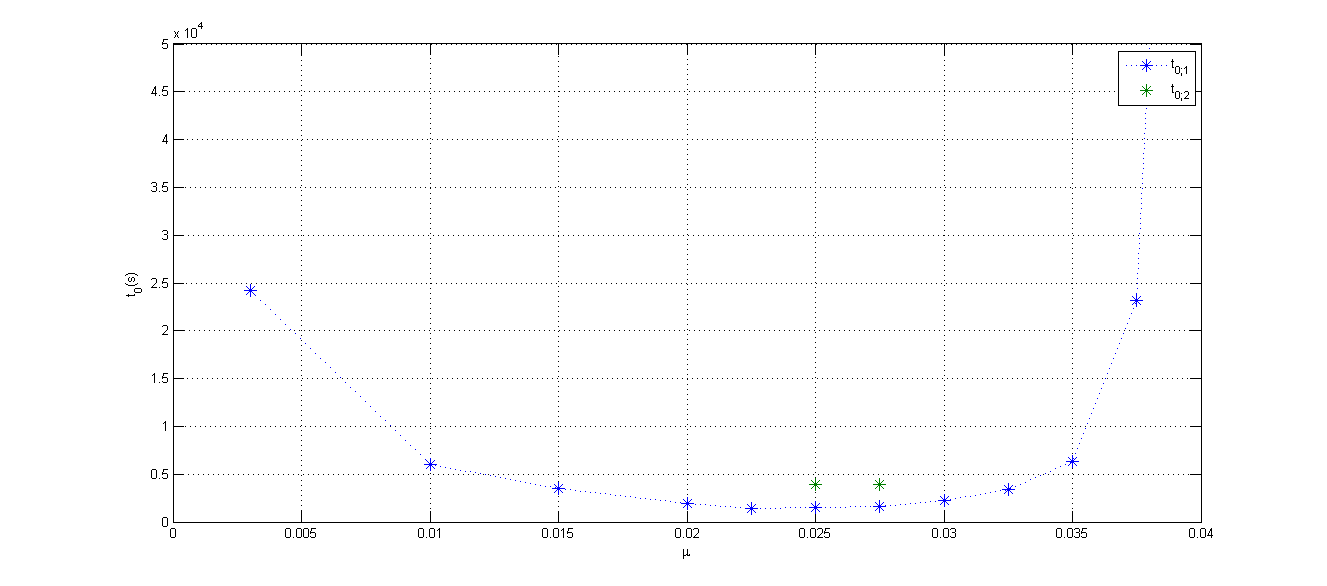
\includegraphics[angle=0,width=1\textwidth]{t0.png}
     \captionof{figure}{ Gráfico tempo de convergência, $t_0$, em função do passo de adaptação, $\mu$. Os pontos a azul são relativos à primeira convergência, e os pontos a verde são relativos à segunda convergência  (casos  $\mu=0.0250$ e $\mu=0.0275$). }
     \label{fig:t0}
     \end{center}

\begin{center}
     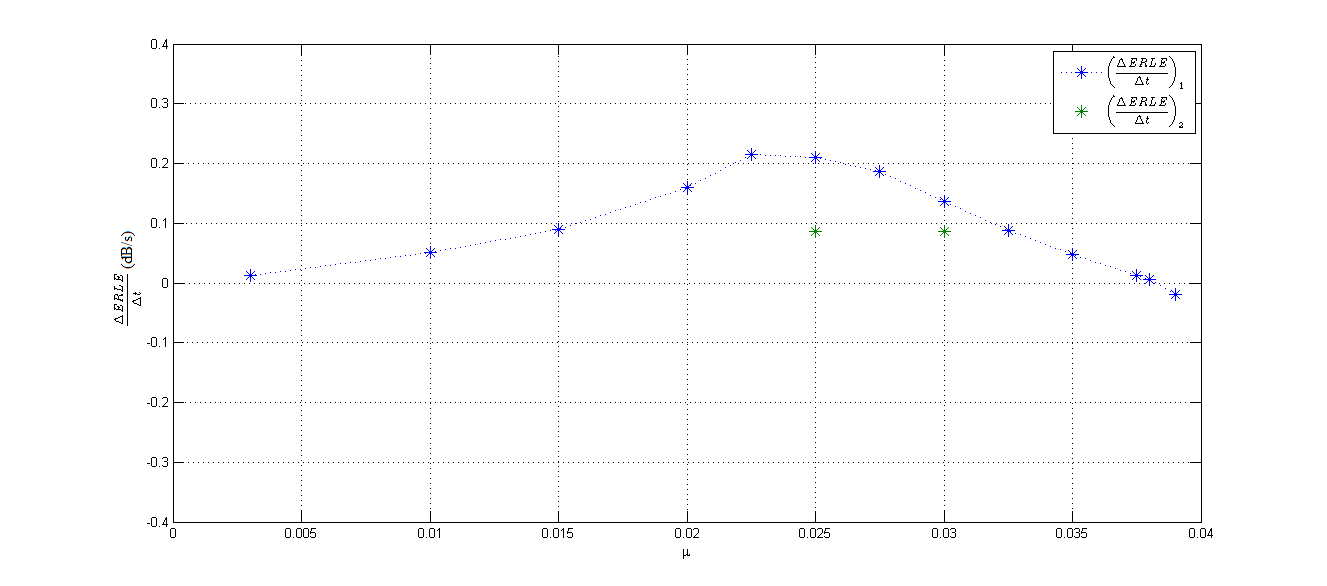
\includegraphics[angle=0,width=1\textwidth]{declive.png}
     \captionof{figure}{ Gráfico declive,  $\frac{\Delta ERLE}{\Delta t}$ ($dB/s$), em função do passo de adaptação, $\mu$. Os pontos a azul são relativos à primeira convergência, e os pontos a verde são relativos à segunda convergência  (casos  $\mu=0.0250$ e $\mu=0.0275$). }
     \label{fig:declive}
     \end{center}
     
\begin{center}
     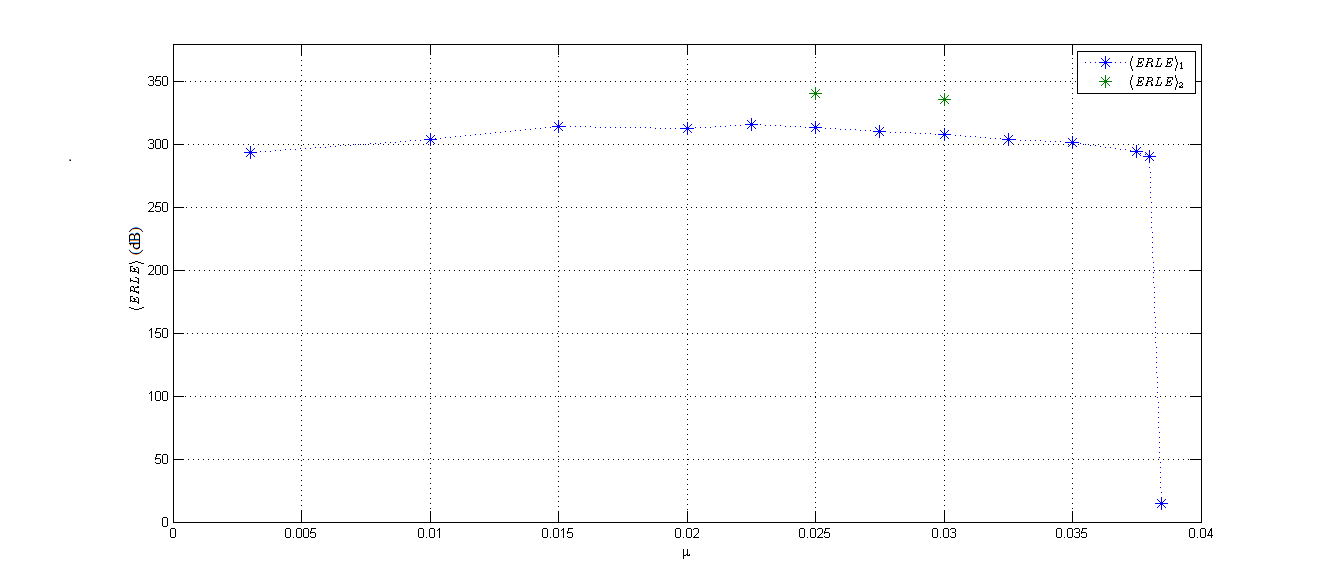
\includegraphics[angle=0,width=1\textwidth]{med.png}
     \captionof{figure}{ Gráfico do valor médio no regime estacionário,  $\langle ERLE_{st} \rangle$ ($dB$), em função do passo de adaptação, $\mu$. Os pontos a azul são relativos à primeira convergência, e os pontos a verde são relativos à segunda convergência  (casos  $\mu=0.0250$ e $\mu=0.0275$). }
     \label{fig:med}
     \end{center}
     
\begin{center}
     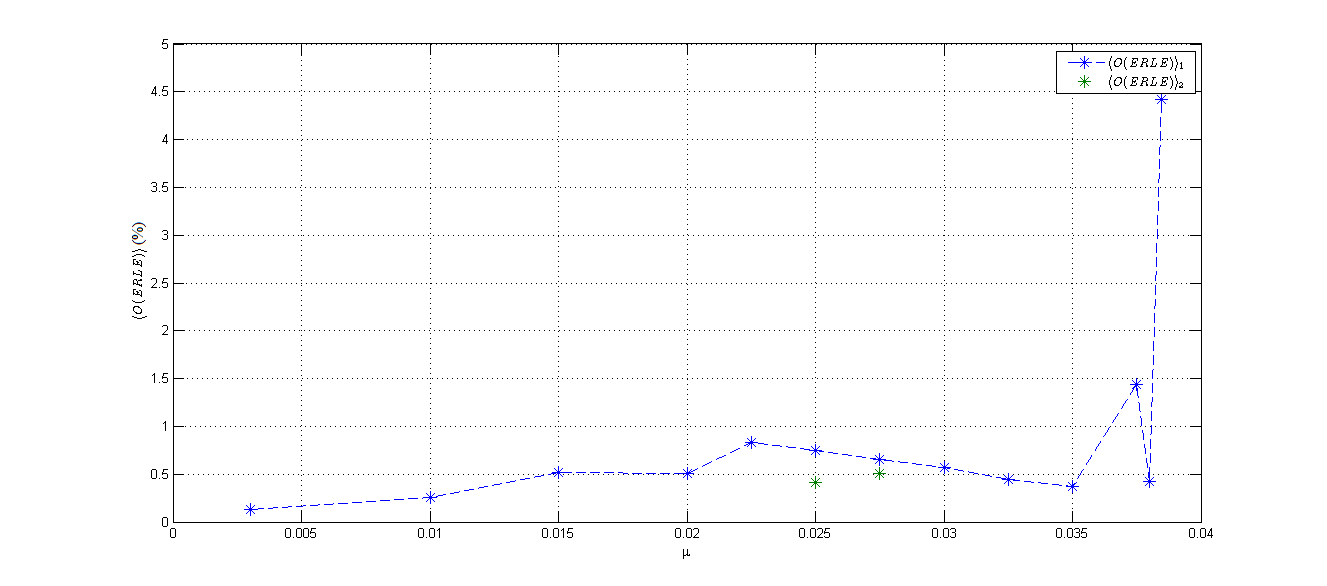
\includegraphics[angle=0,width=1\textwidth]{osc.png}
     \captionof{figure}{ Gráfico valor médio relativo das oscilações no regime estacionário,  $\langle O(ERLE_{st})\rangle_r$(\%), em função do passo de adaptação, $\mu$. Os pontos a azul são relativos à primeira convergência, e os pontos a verde são relativos à segunda convergência  (casos  $\mu=0.0250$ e $\mu=0.0275$). }
     \label{fig:osc}
     \end{center}
     
     
Analisando o gráfico tempo de convergência, $t_0$ em função do passo de adaptação $\mu$ (figura \ref{fig:t0}) pode-se constatar, que este apresenta uma concavidade virada para cima. Existe portanto, um intervalo de optimização do tempo de convergência,  que se considerou ser $u\in[0.02,0.03]$, sendo $t_0$ mínimo para $\mu_{(opt. \hspace{2pt} t_0)}=0.0225$. Verifica-se também que o tempo de convergência explode quando $\mu \to u_c^-$.\\
\par
Relativamente ao gráfico declive $\frac{\Delta ERLE}{\Delta t}$ em função de $\mu$ (figura \ref{fig:declive}), pode-se referir que este apresenta concavidade virada para baixo. Existe  um intervalo de optimização do declive,  que se considerou ser $u\in[0.02,0.03]$, o mesmo que o de optimização do tempo de convergência. Verifica-se um máximo de $\frac{\Delta ERLE}{\Delta t}$ para $\mu_{(opt. \hspace{2pt} \frac{\Delta ERLE}{\Delta t})}=0.0225$, o mesmo valor de $\mu$ que optimiza $t_0$.\\

\par Quanto ao gráfico valor médio no regime estacionário,  $\langle ERLE_{st} \rangle$, em função do passo de adaptação, $\mu$, (figura \ref{fig:med}), pode-se dizer que este é aproximadamente constante. Apresenta um máximo de 1ª convergência em $\mu_{\left({opt. \hspace{2pt} \langle ERLE \rangle}_1\right)}=0.0225$, mesmo valor que os de optimização de $t_o$ e $\frac{\Delta ERLE}{\Delta t}$ e um máximo de 2ª convergência superior à de 1ª, em $\mu_{\left({opt. \hspace{2pt} \langle ERLE \rangle}_2\right)}=0.025$.\\
\par

Analisando o gráfico valor médio relativo das oscilações em regime estacionário,  $\langle O(ERLE_{st})\rangle_r$, em função do passo de adaptação $\mu$ (figura \ref{fig:osc}) conclui-se que este apresenta maiores valores para as zonas de optimização dos outros parâmetros referidos anteriormente, sendo que para $\mu>0.035$ verifica-se um certo comportamento irregular. No entanto, pode-se afirmar que a estabilidade é tanto maior, quanto menor for $\mu$. Da gama de valores $\mu$ que se testou, o que optimiza a estabilidade é $\mu_{\left({opt. \hspace{2pt} \langle O(ERLE) \rangle}\right)}=0.003$. O passo $\mu=0.0225$ que permitia optimizar $t_0$, $\frac{\Delta ERLE}{\Delta t}$ e  $\frac{\Delta ERLE}{\Delta t}$ está associado ao 3º maior máximo relativo do gráfico, sendo o máximo absoluto correspondente ao passo crítico, $\mu_c$, tal como já foi referido anteriormente.\\
\par
\large\underline{{\textit{\textbf{Sugestões de optimização do sistema}}}}\\
\par

Existem 4 parâmetros do sistema que podem ser optimizados: 

\begin{itemize}
\item Tempo de convergência, $t_0$;
\item Rácio $\frac{\Delta ERLE}{\Delta t}$;
\item Valor do $ERLE$ em convergência, $\langle ERLE_{st} \rangle$;
\item Instabilidade, $\langle O(ERLE_{st})\rangle$.
\end{itemize}

Optimizar o tempo de convergência, ou rácio $\frac{\Delta ERLE}{\Delta t}$, implica optimizar ambos, já que o valor do passo de adaptação associado é o mesmo: $\mu_{(opt. \hspace{2pt} t_0)}=\mu_{(opt. \hspace{2pt} \frac{\Delta ERLE}{\Delta t})}=0.0225$. Implica também quase optimizar o valor médio do $ERLE$ em regime estacionário, $\langle ERLE_{st} \rangle$, existindo apenas uma convergência (valor de  $\langle ERLE_{st} \rangle$ para a convergência de 2ª ordem, nos casos de $\mu=0.025$ e $\mu=0.0275$, é superior).\\
\par
Optimizar $\langle ERLE_{st} \rangle$, seria estabelecer $\mu=0.025$ (convergência de 2ª ordem, que abdica da performance em $t_0$ e $\frac{\Delta ERLE}{\Delta t}$ ). Ainda assim, o comportamento do sistema para a convergência de 1ª ordem ($t_{0_1}$,  $\left(\frac{\Delta ERLE}{\Delta t}\right)_1$ $\langle ERLE_{st} \rangle_1$ e $\langle O(ERLE_{st})\rangle_1$) no caso de $\mu=0.025$ é bastante semelhante ao do caso $\mu=0.0225$. \\
\par
A estabilidade pode ser optimizada, escolhendo $\mu$, o mais pequeno possível. No entanto, para  $\mu$ reduzido, nenhum dos outros parâmetro anteriores poderia ser melhorado. Para  $\mu=0.0225$, tem-se uma instabilidade elevada - optimizar a performance do sistema em $t_0$,  $\frac{\Delta ERLE}{\Delta t}$ $ERLE$, e $\langle ERLE_{st} \rangle$ implica o sacrifício da sua estabilidade. Relativamente a  $\mu=0.0250$ tem-se uma maior estabilidade quer para a 1ª convergência, quer para a 2ª.\\
\par
Tendo em conta toda a discussão realizada nos 4 parágrafos anteriores, conclui-se que o valor do passo de adaptação $\mu$ optimizador do sistema é:

$$\mu_{opt}=0.0250$$

ou mais correctamente: 

$$\mu_{opt}\in[0.0225,0.0250]$$

 já que os resultados obtidos foram pontuais (o varrimento de $\mu$ não foi contínuo). Esta escolha teve em consideração, o facto de que para este intervalo de $\mu$, tem-se um bom comportamento do sistema em 1ª convergência e a possibilidade de 2ª convergência que permite o melhoramento, a posteriori, de $\frac{\Delta ERLE}{\Delta t}$ e  $\langle O(ERLE_{st})\rangle$.







\subsection{Teste do sistema com ruído}

\large\underline{{\textit{\textbf{Implementação do passo de adaptação $\mu=0.03$ e $G=0.1$}}}}\\
\par
Pretende-se de seguida analisar o sistema, mas introduzindo ruído ao mesmo para simular condições mais aproximadas do que acontece na vida prática. O ruído vai ser introduzido por meio de um gerador de dados remoto com um ganho G definido previamente. Este gerador é independente do gerador de dados local.

Começou-se por implementar um passo de adaptação $\mu=0.03$, $G=0.1$ e tempo de aquisição, $T=1000s$. Obtiveram-se os gráficos  das evoluções no tempo, do $ERLE$ (figura \ref{fig:SRuRUIDO}) e dos valores dos coeficientes do \textit{Cancelador de Eco}, $c_k$ (figura \ref{fig:SRuRUIDOt}).


\begin{center}
     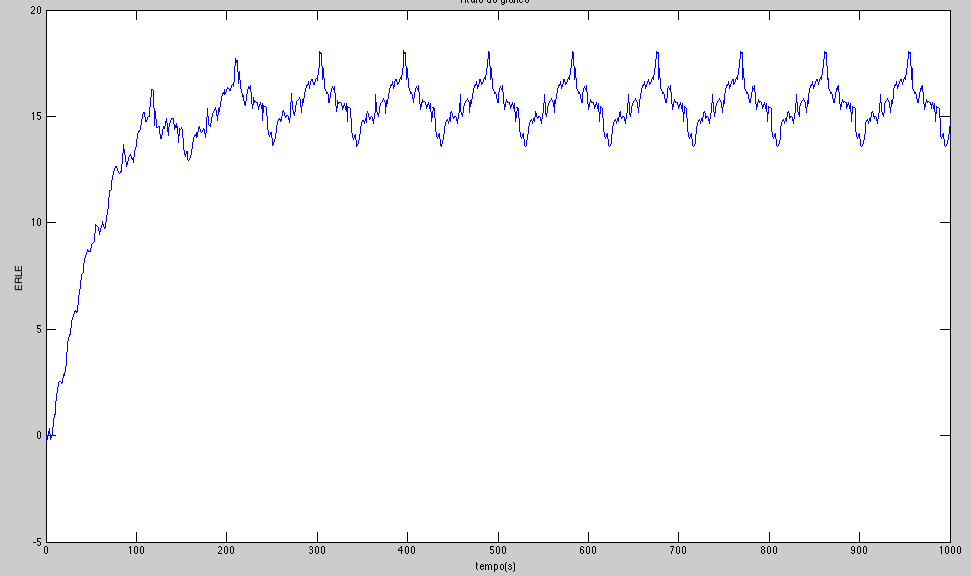
\includegraphics[angle=0,width=1\textwidth]{ERLE_G0_1}
     \captionof{figure}{Gráfico parâmetro de eficiência, $ERLE$, em função do tempo, $t(s)$, para $\mu=0.03$, $G=0.1$ e $T=1000s$.}
     \label{fig:SRuRUIDO}
     \end{center}


\begin{center}
     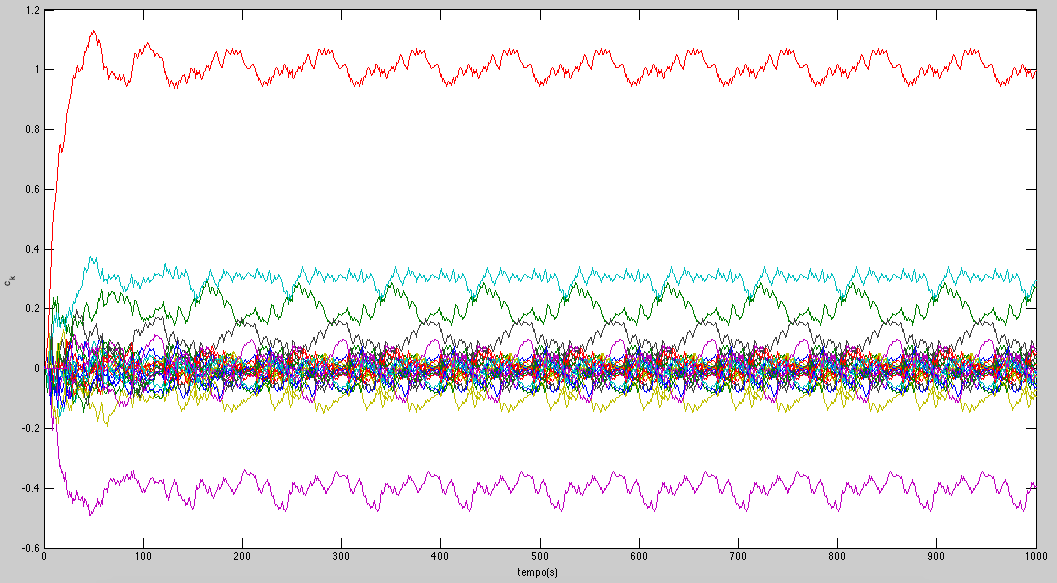
\includegraphics[angle=0,width=1\textwidth]{c_k_G0_1}
     \captionof{figure}{ Gráfico coeficientes $c_k$ em função do tempo, $t(s)$, para $\mu=0.03$, $G=0.1$ e $T=1000s$.}
     \label{fig:SRuRUIDOt}
\end{center}
     
Verifica-se que a introdução de ruído perturba imensamente a atenuação de eco reduzindo o seu valor de cerca de 300dB para 14,71dB. Esta redução pode ser explicada pelo fato de que o cancelador de eco não estar preparada para cancelar ruído, cancelando apenas o eco produzido pelo híbrido. E neste caso o filtro observa o sinal ruído+eco como se apenas de eco se tratasse.

Nesta situação o sinal $e_k$ passa a ser constituído pelo eco e pelo sinal do emissor remoto que, apesar de atenuado, afeta o eco proveniente do emissor local. Posto isto, os coeficientes do filtro adaptativo não vão estabilizar e vão oscilar, periodicamente, em torno de valores médios. Esta oscilação é mais um fator para que o valor do ERLE seja significativamente mais baixo.
\paragraph{}


\large\underline{{\textit{\textbf{Implementação do passo de adaptação $\mu_{máx}$ e $G=0.4$}}}}\\
\par

A figura seguinte representa a evolução temporal do parâmetro ERLE.

\begin{center}
     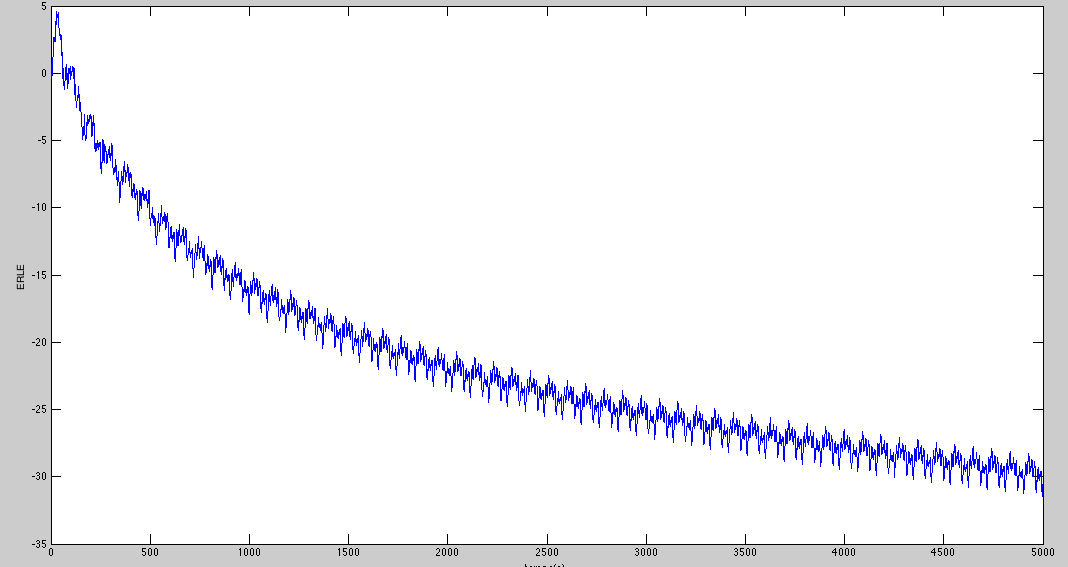
\includegraphics[angle=0,width=0.8\textwidth]{ERLE_G0_4_umax}
     \captionof{figure}{ Gráfico parâmetro de eficiência, $ERLE$, em função do tempo, $t(s)$, para $\mu_{max}$, $G=0.4$ e $T=5000s$.}
     \label{fig:SRuERLEt}
\end{center}

Como é possível constatar o filtro não consegue processar sinais ruidosos levando a valores de ERLE sem significado, falhando na sua função de identificação, e à instabilização dos coeficientes, como é possível visualizar na figura seguinte.

\begin{center}
     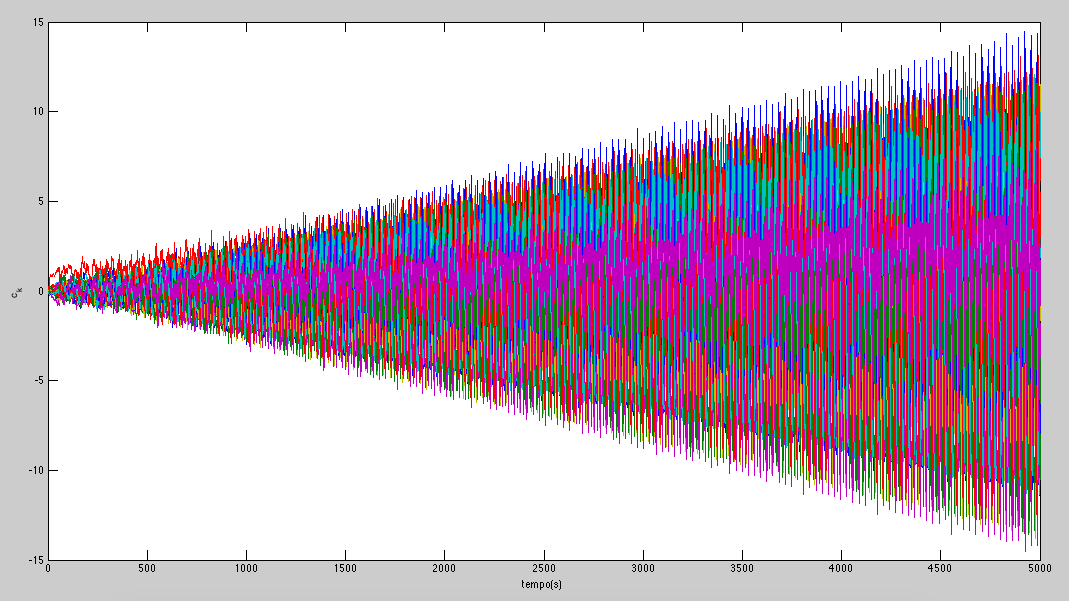
\includegraphics[angle=0,width=0.9\textwidth]{c_k_G0_4_umax}
     \captionof{figure}{ Gráfico coeficientes $c_k$ em função do tempo, $t(s)$, para $\mu_{max}$, $G=0.4$ e $T=5000s$.}
     \label{fig:SRucoeft}
\end{center}

Para resolver esta situação, ou torná-la menos desfavorável, poder-se-ia aumentar a ordem do filtro, mas deve-se notar sempre que não existem sistemas perfeitos e o ruído vai sempre existir e, como tal, é necessário encontrar um ponto de equilíbrio. Outra solução plausível é a alteração dos parâmetros $\mu_{max}$ e/ou a atenuação do ruído que entra no sistema.



\chapter{Conclusões}

Relativamente à simulação do sistema total sem ruído, pode-se referir que a eficiência no cancelamento do eco está intimamente relacionada com o valor do passo de adaptação $\mu$ para o algoritmo $LMS$. Foi possível determinar um intervalo para a optimização do processo, bem como o valor de $\mu$ limite para a sua estabilidade, $\mu_c$. É importante salientar que o sistema, no intervalo de $\mu$ de optimização, apresenta a propriedade de 2ª convergência. Isto significa, que para além dos bons resultados obtidos para a 1ª convergência, é esperado o seu melhoramento na ocorrência da 2ª convergência.\\

Ao testar o sistema com a introdução de ruído, o cancelador de eco vai associar o sinal de erro como proveniente apenas do eco do gerador de dados localquando na realidade ele tem origem também no ruído do emissor remoto. Por outras palavras, vai associar o ruído do gerador remoto ao eco do emissor local e observá-lo como sendo o eco total deste último. Porém, o ruído é independente deste gerador e o filtro apenas vai conseguir identificar correctamente o eco do gerador local sem estabilizar num valor fixo devido ao ruído variável proveniente do emissor remoto. O funcionamento do sistema vai depender ainda do passo de adaptação utilizado. No entanto, para os mesmos valores de $\mu$ utilizados no sistema sem ruído, nota-se uma enorme perda de eficiência e redução do ERLE para $\mu=0,03$. E para $\mu_c$ o sistema fica instável, não cumprindo a sua função.







\end{document}

